% Options for packages loaded elsewhere
\PassOptionsToPackage{unicode}{hyperref}
\PassOptionsToPackage{hyphens}{url}
%
\documentclass[
]{article}
\usepackage{amsmath,amssymb}
\usepackage{lmodern}
\usepackage{iftex}
\ifPDFTeX
  \usepackage[T1]{fontenc}
  \usepackage[utf8]{inputenc}
  \usepackage{textcomp} % provide euro and other symbols
\else % if luatex or xetex
  \usepackage{unicode-math}
  \defaultfontfeatures{Scale=MatchLowercase}
  \defaultfontfeatures[\rmfamily]{Ligatures=TeX,Scale=1}
\fi
% Use upquote if available, for straight quotes in verbatim environments
\IfFileExists{upquote.sty}{\usepackage{upquote}}{}
\IfFileExists{microtype.sty}{% use microtype if available
  \usepackage[]{microtype}
  \UseMicrotypeSet[protrusion]{basicmath} % disable protrusion for tt fonts
}{}
\makeatletter
\@ifundefined{KOMAClassName}{% if non-KOMA class
  \IfFileExists{parskip.sty}{%
    \usepackage{parskip}
  }{% else
    \setlength{\parindent}{0pt}
    \setlength{\parskip}{6pt plus 2pt minus 1pt}}
}{% if KOMA class
  \KOMAoptions{parskip=half}}
\makeatother
\usepackage{xcolor}
\usepackage[margin=1in]{geometry}
\usepackage{color}
\usepackage{fancyvrb}
\newcommand{\VerbBar}{|}
\newcommand{\VERB}{\Verb[commandchars=\\\{\}]}
\DefineVerbatimEnvironment{Highlighting}{Verbatim}{commandchars=\\\{\}}
% Add ',fontsize=\small' for more characters per line
\usepackage{framed}
\definecolor{shadecolor}{RGB}{248,248,248}
\newenvironment{Shaded}{\begin{snugshade}}{\end{snugshade}}
\newcommand{\AlertTok}[1]{\textcolor[rgb]{0.94,0.16,0.16}{#1}}
\newcommand{\AnnotationTok}[1]{\textcolor[rgb]{0.56,0.35,0.01}{\textbf{\textit{#1}}}}
\newcommand{\AttributeTok}[1]{\textcolor[rgb]{0.77,0.63,0.00}{#1}}
\newcommand{\BaseNTok}[1]{\textcolor[rgb]{0.00,0.00,0.81}{#1}}
\newcommand{\BuiltInTok}[1]{#1}
\newcommand{\CharTok}[1]{\textcolor[rgb]{0.31,0.60,0.02}{#1}}
\newcommand{\CommentTok}[1]{\textcolor[rgb]{0.56,0.35,0.01}{\textit{#1}}}
\newcommand{\CommentVarTok}[1]{\textcolor[rgb]{0.56,0.35,0.01}{\textbf{\textit{#1}}}}
\newcommand{\ConstantTok}[1]{\textcolor[rgb]{0.00,0.00,0.00}{#1}}
\newcommand{\ControlFlowTok}[1]{\textcolor[rgb]{0.13,0.29,0.53}{\textbf{#1}}}
\newcommand{\DataTypeTok}[1]{\textcolor[rgb]{0.13,0.29,0.53}{#1}}
\newcommand{\DecValTok}[1]{\textcolor[rgb]{0.00,0.00,0.81}{#1}}
\newcommand{\DocumentationTok}[1]{\textcolor[rgb]{0.56,0.35,0.01}{\textbf{\textit{#1}}}}
\newcommand{\ErrorTok}[1]{\textcolor[rgb]{0.64,0.00,0.00}{\textbf{#1}}}
\newcommand{\ExtensionTok}[1]{#1}
\newcommand{\FloatTok}[1]{\textcolor[rgb]{0.00,0.00,0.81}{#1}}
\newcommand{\FunctionTok}[1]{\textcolor[rgb]{0.00,0.00,0.00}{#1}}
\newcommand{\ImportTok}[1]{#1}
\newcommand{\InformationTok}[1]{\textcolor[rgb]{0.56,0.35,0.01}{\textbf{\textit{#1}}}}
\newcommand{\KeywordTok}[1]{\textcolor[rgb]{0.13,0.29,0.53}{\textbf{#1}}}
\newcommand{\NormalTok}[1]{#1}
\newcommand{\OperatorTok}[1]{\textcolor[rgb]{0.81,0.36,0.00}{\textbf{#1}}}
\newcommand{\OtherTok}[1]{\textcolor[rgb]{0.56,0.35,0.01}{#1}}
\newcommand{\PreprocessorTok}[1]{\textcolor[rgb]{0.56,0.35,0.01}{\textit{#1}}}
\newcommand{\RegionMarkerTok}[1]{#1}
\newcommand{\SpecialCharTok}[1]{\textcolor[rgb]{0.00,0.00,0.00}{#1}}
\newcommand{\SpecialStringTok}[1]{\textcolor[rgb]{0.31,0.60,0.02}{#1}}
\newcommand{\StringTok}[1]{\textcolor[rgb]{0.31,0.60,0.02}{#1}}
\newcommand{\VariableTok}[1]{\textcolor[rgb]{0.00,0.00,0.00}{#1}}
\newcommand{\VerbatimStringTok}[1]{\textcolor[rgb]{0.31,0.60,0.02}{#1}}
\newcommand{\WarningTok}[1]{\textcolor[rgb]{0.56,0.35,0.01}{\textbf{\textit{#1}}}}
\usepackage{longtable,booktabs,array}
\usepackage{calc} % for calculating minipage widths
% Correct order of tables after \paragraph or \subparagraph
\usepackage{etoolbox}
\makeatletter
\patchcmd\longtable{\par}{\if@noskipsec\mbox{}\fi\par}{}{}
\makeatother
% Allow footnotes in longtable head/foot
\IfFileExists{footnotehyper.sty}{\usepackage{footnotehyper}}{\usepackage{footnote}}
\makesavenoteenv{longtable}
\usepackage{graphicx}
\makeatletter
\def\maxwidth{\ifdim\Gin@nat@width>\linewidth\linewidth\else\Gin@nat@width\fi}
\def\maxheight{\ifdim\Gin@nat@height>\textheight\textheight\else\Gin@nat@height\fi}
\makeatother
% Scale images if necessary, so that they will not overflow the page
% margins by default, and it is still possible to overwrite the defaults
% using explicit options in \includegraphics[width, height, ...]{}
\setkeys{Gin}{width=\maxwidth,height=\maxheight,keepaspectratio}
% Set default figure placement to htbp
\makeatletter
\def\fps@figure{htbp}
\makeatother
\setlength{\emergencystretch}{3em} % prevent overfull lines
\providecommand{\tightlist}{%
  \setlength{\itemsep}{0pt}\setlength{\parskip}{0pt}}
\setcounter{secnumdepth}{-\maxdimen} % remove section numbering
\ifLuaTeX
  \usepackage{selnolig}  % disable illegal ligatures
\fi
\IfFileExists{bookmark.sty}{\usepackage{bookmark}}{\usepackage{hyperref}}
\IfFileExists{xurl.sty}{\usepackage{xurl}}{} % add URL line breaks if available
\urlstyle{same} % disable monospaced font for URLs
\hypersetup{
  pdftitle={Enriching a Microbiome Analysis},
  pdfauthor={Thomaz F. S. Bastiaanssen},
  hidelinks,
  pdfcreator={LaTeX via pandoc}}

\title{Enriching a Microbiome Analysis}
\author{Thomaz F. S. Bastiaanssen}
\date{}

\begin{document}
\maketitle

\hypertarget{introduction}{%
\section{0. Introduction}\label{introduction}}

Here, we will demonstrate four strategies to enrich microbiome-gut-brain
axis experiments. In this document we expand on the demonstration in the
supplementary files of the companion piece to this manuscript. We
strongly recommend readers go through that analysis before this
document, for the sake of continuity and clarity.

For this demonstration, we have adapted some shotgun metagenomic data
from the \texttt{curatedMetagenomicData} library in R. We're looking at
a human cohort starring in the \emph{Metagenome-wide association of gut
microbiome features for schizophrenia} study (DOI:
10.1038/s41467-020-15457-9). After downloading the data it was
simplified by summing together all strains by genus. This will make it
easier to analyse without access to a server. For the set of operations
used to pre-process, please see section
\href{https://github.com/thomazbastiaanssen/Tjazi/blob/master/guidebook_sup/part2/README_part2.md\#gathering-and-preparing-our-data-1}{Download
and pre-process microbiome data} in this document. Briefly, in this data
set, we have WGS data from faecal samples from both patients with
schizophrenia and healthy volunteers, which will be referred to as
``healthy'' in the Legends. This data has been included in the
\texttt{Tjazi} library on github for easy access purposes. All R code
used to transform, wrangle (reorganise) and plot the data is also shown
below as to hopefully provide a toolkit for aspiring and veteran
bioinformaticians alike.

\hypertarget{code-chunk-load-our-libraries}{%
\subsubsection{Code chunk: Load our
libraries}\label{code-chunk-load-our-libraries}}

\begin{Shaded}
\begin{Highlighting}[]
\CommentTok{\#Statistical tools        Primarily the CLR transformation.}
\FunctionTok{library}\NormalTok{(Tjazi)            }\CommentTok{\#devtools::install\_github("thomazbastiaanssen/Tjazi")}

\CommentTok{\#Data Wrangling}
\FunctionTok{library}\NormalTok{(tidyverse)        }\CommentTok{\#install.packages("tidyverse")}
\FunctionTok{library}\NormalTok{(knitr)            }\CommentTok{\#install.packages("knitr")}

\CommentTok{\#Plotting}
\FunctionTok{library}\NormalTok{(ggplot2)          }\CommentTok{\#install.packages("ggplot2")}
\FunctionTok{library}\NormalTok{(ggforce)          }\CommentTok{\#install.packages("ggforce")}
\FunctionTok{library}\NormalTok{(patchwork)        }\CommentTok{\#install.packages("patchwork")}

\CommentTok{\#Section specific packages}
\FunctionTok{library}\NormalTok{(mediation)        }\CommentTok{\#install.packages("mediation")}
\FunctionTok{library}\NormalTok{(anansi)           }\CommentTok{\#devtools::install\_github("thomazbastiaanssen/anansi")}
\FunctionTok{library}\NormalTok{(propr)            }\CommentTok{\#devtools::install\_github("tpq/propr")}
\FunctionTok{library}\NormalTok{(volatility)       }\CommentTok{\#devtools::install\_github("thomazbastiaanssen/volatility")}


\CommentTok{\#Load prepared data from the schizophrenia study stored in the Tjazi library}
\FunctionTok{data}\NormalTok{(guidebook\_data)}
\end{Highlighting}
\end{Shaded}

\newpage

\hypertarget{mediation-analysis}{%
\section{1. Mediation analysis}\label{mediation-analysis}}

Mediation analysis is a statistical tool that can help us answer causal
questions. Mediation analysis can be used to address core questions in
the microbiome-gut-brain axis field. One common and important example is
as follows:

\begin{itemize}
\tightlist
\item
  We know diet affects mental health.
\item
  We also know diet affects the microbiome.
\item
  We have observed associations between microbial taxa and mental
  health.
\end{itemize}

But how do we make sure that the association between the microbiome and
mental health isn't due to the fact that they share a common `driver',
namely diet, rendering our observed associations between the microbiome
and the brain merely spurious? Conversely, mediation analysis could help
us find to which degree the underlying mechanism of the effect of diet
on mental health is due to the effect of diet on the microbiome.

Here, we will demonstrate how one could go about performing mediation
analysis to ask and answer this question. We will use the 2020
schizophrenia data set to demonstrate this point. It should be noted
here that in reality, one would need strong biological mechanistic
reasons to perform a mediation analysis in order to make the `causal'
part in causal mediation analysis carry any meaning. Here we are just
performing the analysis for demonstrative purposes.

\hypertarget{gathering-and-preparing-our-data}{%
\subsection{Gathering and preparing our
data}\label{gathering-and-preparing-our-data}}

First, Let's load the schizophrenia data set into our environment. We'll
also quickly clean and CLR-transform our genus-level count table.

\hypertarget{code-chunk-preparing-microbiome-data}{%
\subsubsection{Code chunk: Preparing microbiome
data}\label{code-chunk-preparing-microbiome-data}}

\begin{Shaded}
\begin{Highlighting}[]
\CommentTok{\#Set a seed for the purposes of reproducibility in this document.}
\FunctionTok{set.seed}\NormalTok{(}\DecValTok{1}\NormalTok{)}

\CommentTok{\#Load the mediation library and the relevant files for demo}
\FunctionTok{library}\NormalTok{(mediation)}
\FunctionTok{data}\NormalTok{(guidebook\_data)}
\NormalTok{counts   }\OtherTok{\textless{}{-}}\NormalTok{ counts ; metadata }\OtherTok{\textless{}{-}}\NormalTok{ metadata ; diet }\OtherTok{\textless{}{-}}\NormalTok{ diet}

\CommentTok{\#Repeat the cleaning and transformation steps from part 1}
\NormalTok{metadata}\SpecialCharTok{$}\NormalTok{master\_ID }\OtherTok{\textless{}{-}} \FunctionTok{gsub}\NormalTok{(metadata}\SpecialCharTok{$}\NormalTok{master\_ID, }\AttributeTok{pattern =} \StringTok{"{-}"}\NormalTok{, }\AttributeTok{replacement =} \StringTok{"."}\NormalTok{)}

\NormalTok{counts  }\OtherTok{\textless{}{-}}\NormalTok{ counts[,metadata}\SpecialCharTok{$}\NormalTok{master\_ID]}

\CommentTok{\#Fork off your count data so that you always have an untouched version handy.}
\NormalTok{genus   }\OtherTok{\textless{}{-}}\NormalTok{ counts}

\CommentTok{\#make sure our count data is all numbers}
\NormalTok{genus   }\OtherTok{\textless{}{-}} \FunctionTok{apply}\NormalTok{(genus,}\FunctionTok{c}\NormalTok{(}\DecValTok{1}\NormalTok{,}\DecValTok{2}\NormalTok{),}\ControlFlowTok{function}\NormalTok{(x) }\FunctionTok{as.numeric}\NormalTok{(}\FunctionTok{as.character}\NormalTok{(x)))}

\CommentTok{\#Remove features with prevalence \textless{} 10\% in two steps:}
\CommentTok{\#First, determine how often every feature is absent in a sample}
\NormalTok{n\_zeroes }\OtherTok{\textless{}{-}} \FunctionTok{rowSums}\NormalTok{(genus }\SpecialCharTok{==} \DecValTok{0}\NormalTok{)}

\CommentTok{\#Then, remove features that are absent in more than your threshold (90\% in this case).}
\NormalTok{genus    }\OtherTok{\textless{}{-}}\NormalTok{ genus[n\_zeroes }\SpecialCharTok{\textless{}=} \FunctionTok{round}\NormalTok{(}\FunctionTok{ncol}\NormalTok{(genus) }\SpecialCharTok{*} \FloatTok{0.90}\NormalTok{),]}

\CommentTok{\#Perform a CLR transformation}
\NormalTok{genus.exp }\OtherTok{\textless{}{-}} \FunctionTok{clr\_c}\NormalTok{(genus)}
\end{Highlighting}
\end{Shaded}

\hypertarget{preparing-the-dietary-data}{%
\subsection{Preparing the dietary
data}\label{preparing-the-dietary-data}}

Furthermore, we will need to prepare the dietary data. For this study,
we have access to a table of five columns denoting how frequently our
participants eat food groups. It should be noted that we are only using
this data for demonstration purposes. In reality, the resolution of the
dietary information provided with this study would not be sufficient to
make any type of causal claim for several reasons. That said, let's
convert the dietary frequency categories into numbers and then perform a
principal component analysis.

\hypertarget{code-chunk-preparing-dietary-data}{%
\subsubsection{Code chunk: Preparing dietary
data}\label{code-chunk-preparing-dietary-data}}

\begin{Shaded}
\begin{Highlighting}[]
\NormalTok{diet.pca }\OtherTok{=}\NormalTok{ diet }\SpecialCharTok{\%\textgreater{}\%} 
  
\CommentTok{\#Replace text with numbers}
  \FunctionTok{mutate}\NormalTok{(}\FunctionTok{across}\NormalTok{(}\FunctionTok{everything}\NormalTok{(), }\SpecialCharTok{\textasciitilde{}}\FunctionTok{str\_replace}\NormalTok{( ., }\StringTok{"hardly"}\NormalTok{,                      }\StringTok{"1"}\NormalTok{ )),}
         \FunctionTok{across}\NormalTok{(}\FunctionTok{everything}\NormalTok{(), }\SpecialCharTok{\textasciitilde{}}\FunctionTok{str\_replace}\NormalTok{( ., }\StringTok{"often"}\NormalTok{,                       }\StringTok{"2"}\NormalTok{ )),}
         \FunctionTok{across}\NormalTok{(}\FunctionTok{everything}\NormalTok{(), }\SpecialCharTok{\textasciitilde{}}\FunctionTok{str\_replace}\NormalTok{( ., }\StringTok{"twice or three times a week"}\NormalTok{, }\StringTok{"3"}\NormalTok{ )),}
         \FunctionTok{across}\NormalTok{(}\FunctionTok{everything}\NormalTok{(), }\SpecialCharTok{\textasciitilde{}}\FunctionTok{str\_replace}\NormalTok{( ., }\StringTok{"every day"}\NormalTok{,                   }\StringTok{"4"}\NormalTok{ )), }
         \FunctionTok{across}\NormalTok{(}\FunctionTok{everything}\NormalTok{(), as.numeric)) }\SpecialCharTok{\%\textgreater{}\%} 

\CommentTok{\#Center and rescale data, then perform a principal component analysis}
  \FunctionTok{scale}\NormalTok{() }\SpecialCharTok{\%\textgreater{}\%}   
  \FunctionTok{prcomp}\NormalTok{()       }

\CommentTok{\#Let\textquotesingle{}s check out the loadings of the first principal component using a histogram }
\NormalTok{PC1 }\OtherTok{=}\NormalTok{ diet.pca}\SpecialCharTok{$}\NormalTok{x[,}\DecValTok{1}\NormalTok{]}
\FunctionTok{hist}\NormalTok{(PC1)}
\end{Highlighting}
\end{Shaded}

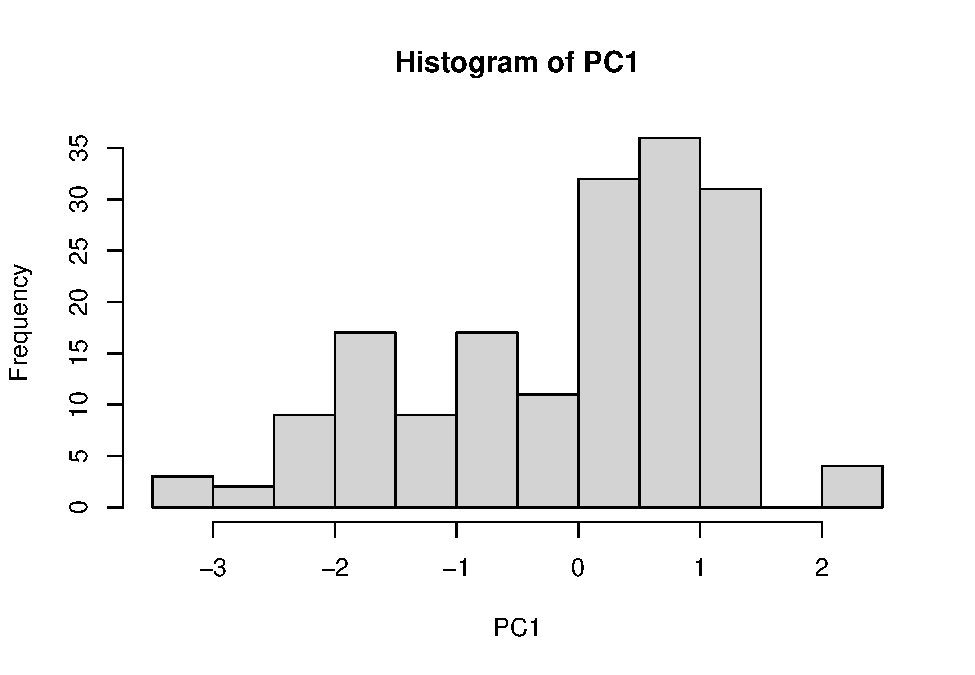
\includegraphics{README_part2_files/figure-latex/diet_pca-1.pdf}

It's always a good idea to visually inspect your data. From this
histogram, it looks like there may be two roughly normal populations in
our first principal component. We'll take note of this and proceed with
our preparations.

\hypertarget{prepare-data-for-mediation-analysis}{%
\subsection{Prepare data for mediation
analysis}\label{prepare-data-for-mediation-analysis}}

We'll take two of the bacteria, \emph{Cronobacter} and
\emph{Gordonibacter}, that were found to be statistically associated
with schizophrenia in our initial analysis. We'll also take the first
component of the dietary intake PCA we generated above.

\hypertarget{code-chunk-preparing-for-mediation-analysis}{%
\subsubsection{Code chunk: Preparing for mediation
analysis}\label{code-chunk-preparing-for-mediation-analysis}}

\begin{Shaded}
\begin{Highlighting}[]
\NormalTok{df\_mediation }\OtherTok{\textless{}{-}} \FunctionTok{data.frame}\NormalTok{(}
  \AttributeTok{Cronobacter    =} \FunctionTok{unlist}\NormalTok{(genus.exp[}\StringTok{"Enterobacteriaceae\_Cronobacter"}\NormalTok{,]),}
  \AttributeTok{Gordonibacter  =} \FunctionTok{unlist}\NormalTok{(genus.exp[}\StringTok{"Eggerthellaceae\_Gordonibacter"}\NormalTok{,]),}
  \AttributeTok{diet\_PC1       =}\NormalTok{ PC1, }
  \AttributeTok{phenotype      =}\NormalTok{ metadata}\SpecialCharTok{$}\NormalTok{Group }\SpecialCharTok{==} \StringTok{"schizophrenia"}\NormalTok{)}
\end{Highlighting}
\end{Shaded}

\newpage

\hypertarget{fit-models}{%
\subsection{Fit models}\label{fit-models}}

For mediation analysis, we need to consider a few models. Microbes will
be playing the role of (potential) mediator here.

\begin{itemize}
\item
  First, we estimate the effect of diet on our phenotype:
  \(phenotype \sim diet\). Does diet explain phenotype? If yes, we can
  proceed.
\item
  Second, we estimate the effect of the microbe on our phenotype of
  interest: \(phenotype \sim microbe\). Does the microbe also explain
  phenotype? If also yes, great, we have a potential mediation on our
  hands.
\item
  Third, we estimate the effect of diet on our microbe of interest:
  \(microbe \sim diet\). Does diet explain the abundance of our microbe?
  If yes, we can proceed. Now things are getting interesting as we have
  the scenario we laid out earlier.
\item
  Fourth, we estimate the \emph{joint} effect of diet and the microbe on
  our phenotype of interest: \(phenotype \sim diet + microbe\). Does
  diet now explain phenotype worse in the presence of the microbe? If
  so, we have a potential mediation on our hands. In the case that diet
  no longer explains phenotype at all, we may be dealing with a full
  mediation. in the case of a reduction of explanatory potential, we
  rather speak of a potential partial mediation.
\end{itemize}

To check for a mediation effect, we use the \texttt{mediation} package.

In our case, the phenotype (schizophrenia diagnosis) is a binary
outcome. Because of that, we'll use a logistic regression model rather
than a `regular' linear model whenever we're trying to explain
phenotype. We'll use a link function for this.

Let's give it a shot with our two bacteria.

\hypertarget{code-chunk-fitting-statistical-models}{%
\subsubsection{Code chunk: Fitting statistical
models}\label{code-chunk-fitting-statistical-models}}

\begin{Shaded}
\begin{Highlighting}[]
\CommentTok{\#Cronobacter}
\CommentTok{\#Does diet explain phenotype?}
\NormalTok{diet.fit1  }\OtherTok{\textless{}{-}} \FunctionTok{glm}\NormalTok{(phenotype }\SpecialCharTok{\textasciitilde{}}\NormalTok{ diet\_PC1, }
                  \AttributeTok{family =} \FunctionTok{binomial}\NormalTok{(}\StringTok{"logit"}\NormalTok{), }\AttributeTok{data =}\NormalTok{ df\_mediation)}

\CommentTok{\#Does diet explain Cronobacter?}
\NormalTok{diba.fit1  }\OtherTok{\textless{}{-}}  \FunctionTok{lm}\NormalTok{(Cronobacter }\SpecialCharTok{\textasciitilde{}}\NormalTok{ diet\_PC1, }\AttributeTok{data =}\NormalTok{ df\_mediation)}

\CommentTok{\#Does Gordonibacter explain phenotype?}
\NormalTok{bact.fit1  }\OtherTok{\textless{}{-}}  \FunctionTok{glm}\NormalTok{(phenotype }\SpecialCharTok{\textasciitilde{}}\NormalTok{ Cronobacter, }
                    \AttributeTok{family =} \FunctionTok{binomial}\NormalTok{(}\StringTok{"logit"}\NormalTok{), }\AttributeTok{data =}\NormalTok{ df\_mediation)}

\CommentTok{\#Does diet explain phenotype on the presence of Cronobacter?}
\NormalTok{both.fit1  }\OtherTok{\textless{}{-}} \FunctionTok{glm}\NormalTok{(phenotype }\SpecialCharTok{\textasciitilde{}}\NormalTok{ diet\_PC1 }\SpecialCharTok{+}\NormalTok{ Cronobacter, }
                  \AttributeTok{family =} \FunctionTok{binomial}\NormalTok{(}\StringTok{"logit"}\NormalTok{), }\AttributeTok{data =}\NormalTok{ df\_mediation)}

\CommentTok{\#Is there a mediation effect here?}
\NormalTok{crono }\OtherTok{=} \FunctionTok{mediate}\NormalTok{(diba.fit1, both.fit1, }
                \AttributeTok{treat =} \StringTok{\textquotesingle{}diet\_PC1\textquotesingle{}}\NormalTok{, }\AttributeTok{mediator =} \StringTok{\textquotesingle{}Cronobacter\textquotesingle{}}\NormalTok{, }\AttributeTok{boot =}\NormalTok{ T)}
\end{Highlighting}
\end{Shaded}

\begin{verbatim}
## Running nonparametric bootstrap
\end{verbatim}

\begin{Shaded}
\begin{Highlighting}[]
\CommentTok{\#Gordonibacter}
\CommentTok{\#Does diet explain phenotype?}
\NormalTok{diet.fit2  }\OtherTok{\textless{}{-}} \FunctionTok{glm}\NormalTok{(phenotype }\SpecialCharTok{\textasciitilde{}}\NormalTok{ diet\_PC1, }
                  \AttributeTok{family =} \FunctionTok{binomial}\NormalTok{(}\StringTok{"logit"}\NormalTok{), }\AttributeTok{data =}\NormalTok{ df\_mediation)}

\CommentTok{\#Does diet explain Gordonibacter?}
\NormalTok{diba.fit2  }\OtherTok{\textless{}{-}}  \FunctionTok{lm}\NormalTok{(Gordonibacter }\SpecialCharTok{\textasciitilde{}}\NormalTok{ diet\_PC1, }\AttributeTok{data =}\NormalTok{ df\_mediation)}

\CommentTok{\#Does Gordonibacter explain phenotype?}
\NormalTok{bact.fit2  }\OtherTok{\textless{}{-}}  \FunctionTok{glm}\NormalTok{(phenotype }\SpecialCharTok{\textasciitilde{}}\NormalTok{ Gordonibacter, }
                    \AttributeTok{family =} \FunctionTok{binomial}\NormalTok{(}\StringTok{"logit"}\NormalTok{), }\AttributeTok{data =}\NormalTok{ df\_mediation)}

\CommentTok{\#Does diet explain phenotype on the presence of Gordonibacter?}
\NormalTok{both.fit2  }\OtherTok{\textless{}{-}} \FunctionTok{glm}\NormalTok{(phenotype }\SpecialCharTok{\textasciitilde{}}\NormalTok{ diet\_PC1 }\SpecialCharTok{+}\NormalTok{ Gordonibacter, }
                  \AttributeTok{family =} \FunctionTok{binomial}\NormalTok{(}\StringTok{"logit"}\NormalTok{), }\AttributeTok{data =}\NormalTok{ df\_mediation)}

\CommentTok{\#Is there a mediation effect here?}
\NormalTok{gordo }\OtherTok{=} \FunctionTok{mediate}\NormalTok{(diba.fit2, both.fit2, }
                \AttributeTok{treat =} \StringTok{\textquotesingle{}diet\_PC1\textquotesingle{}}\NormalTok{, }\AttributeTok{mediator =} \StringTok{\textquotesingle{}Gordonibacter\textquotesingle{}}\NormalTok{, }\AttributeTok{boot =}\NormalTok{ T)}
\end{Highlighting}
\end{Shaded}

\begin{verbatim}
## Running nonparametric bootstrap
\end{verbatim}

Notice that in the \texttt{mediate} function calls, we're essentially
estimating the explanatory potential of diet on our phenotype, in the
presence of our bacteria, in light of the fact that diet also explains
our bacterial abundance.

\newpage

\hypertarget{investigate-results}{%
\subsection{Investigate results}\label{investigate-results}}

Let's take a look at the model summaries. We've picked the first
bacterium, \emph{Cronobacter}, to display a statistically significant
mediation effect.

\hypertarget{code-chunk-cronobacter-results}{%
\subsubsection{Code chunk: Cronobacter
results}\label{code-chunk-cronobacter-results}}

\begin{Shaded}
\begin{Highlighting}[]
\CommentTok{\#Collect the relevant data to display in tables}
\NormalTok{res\_diet.fit1 }\OtherTok{\textless{}{-}} \FunctionTok{coefficients}\NormalTok{(}\FunctionTok{summary}\NormalTok{(diet.fit1))}
\NormalTok{res\_diba.fit1 }\OtherTok{\textless{}{-}} \FunctionTok{coefficients}\NormalTok{(}\FunctionTok{summary}\NormalTok{(diba.fit1))}
\NormalTok{res\_bact.fit1 }\OtherTok{\textless{}{-}} \FunctionTok{coefficients}\NormalTok{(}\FunctionTok{summary}\NormalTok{(bact.fit1))}
\NormalTok{res\_both.fit1 }\OtherTok{\textless{}{-}} \FunctionTok{coefficients}\NormalTok{(}\FunctionTok{summary}\NormalTok{(both.fit1))}
                      
\CommentTok{\#Plot the results in nice looking tables:}
\FunctionTok{kable}\NormalTok{(res\_diet.fit1, }\AttributeTok{digits =} \DecValTok{3}\NormalTok{, }
      \AttributeTok{caption =} \StringTok{"Diet significantly explains phenotype (Estimate of 0.241)."}\NormalTok{)}
\end{Highlighting}
\end{Shaded}

\begin{longtable}[]{@{}lrrrr@{}}
\caption{Diet significantly explains phenotype (Estimate of
0.241).}\tabularnewline
\toprule()
& Estimate & Std. Error & z value &
Pr(\textgreater\textbar z\textbar) \\
\midrule()
\endfirsthead
\toprule()
& Estimate & Std. Error & z value &
Pr(\textgreater\textbar z\textbar) \\
\midrule()
\endhead
(Intercept) & 0.106 & 0.155 & 0.687 & 0.492 \\
diet\_PC1 & 0.241 & 0.122 & 1.972 & 0.049 \\
\bottomrule()
\end{longtable}

\begin{Shaded}
\begin{Highlighting}[]
\FunctionTok{kable}\NormalTok{(res\_diba.fit1, }\AttributeTok{digits =} \DecValTok{3}\NormalTok{, }
      \AttributeTok{caption =} \StringTok{"Diet significantly explains Cronobacter."}\NormalTok{)}
\end{Highlighting}
\end{Shaded}

\begin{longtable}[]{@{}lrrrr@{}}
\caption{Diet significantly explains Cronobacter.}\tabularnewline
\toprule()
& Estimate & Std. Error & t value &
Pr(\textgreater\textbar t\textbar) \\
\midrule()
\endfirsthead
\toprule()
& Estimate & Std. Error & t value &
Pr(\textgreater\textbar t\textbar) \\
\midrule()
\endhead
(Intercept) & -2.461 & 0.114 & -21.676 & 0.000 \\
diet\_PC1 & 0.182 & 0.088 & 2.061 & 0.041 \\
\bottomrule()
\end{longtable}

\begin{Shaded}
\begin{Highlighting}[]
\FunctionTok{kable}\NormalTok{(res\_bact.fit1, }\AttributeTok{digits =} \DecValTok{3}\NormalTok{, }
      \AttributeTok{caption =} \StringTok{"Cronobacter significantly explains phenotype. This comes as }
\StringTok{      no surprise as saw this in our initial differential abundance analysis."}\NormalTok{)}
\end{Highlighting}
\end{Shaded}

\begin{longtable}[]{@{}lrrrr@{}}
\caption{Cronobacter significantly explains phenotype. This comes as no
surprise as saw this in our initial differential abundance
analysis.}\tabularnewline
\toprule()
& Estimate & Std. Error & z value &
Pr(\textgreater\textbar z\textbar) \\
\midrule()
\endfirsthead
\toprule()
& Estimate & Std. Error & z value &
Pr(\textgreater\textbar z\textbar) \\
\midrule()
\endhead
(Intercept) & 0.882 & 0.332 & 2.655 & 0.008 \\
Cronobacter & 0.310 & 0.114 & 2.722 & 0.006 \\
\bottomrule()
\end{longtable}

\begin{Shaded}
\begin{Highlighting}[]
\FunctionTok{kable}\NormalTok{(res\_both.fit1, }\AttributeTok{digits =} \DecValTok{3}\NormalTok{, }
      \AttributeTok{caption =} \StringTok{"In the presence of Cronobacter, diet significantly }
\StringTok{      explains phenotype less well (Estimate of 0.199)."}\NormalTok{)}
\end{Highlighting}
\end{Shaded}

\begin{longtable}[]{@{}lrrrr@{}}
\caption{In the presence of Cronobacter, diet significantly explains
phenotype less well (Estimate of 0.199).}\tabularnewline
\toprule()
& Estimate & Std. Error & z value &
Pr(\textgreater\textbar z\textbar) \\
\midrule()
\endfirsthead
\toprule()
& Estimate & Std. Error & z value &
Pr(\textgreater\textbar z\textbar) \\
\midrule()
\endhead
(Intercept) & 0.831 & 0.337 & 2.467 & 0.014 \\
diet\_PC1 & 0.199 & 0.124 & 1.601 & 0.109 \\
Cronobacter & 0.288 & 0.115 & 2.496 & 0.013 \\
\bottomrule()
\end{longtable}

Looks like we may have a mediation effect here, so let's check out the
results of our mediation analysis: ACME stands for Average Causal
Mediation Effect, whereas ADE stands for Average Direct Effect.

\hypertarget{code-chunk-cronobacter-mediation-figure}{%
\subsubsection{Code chunk: Cronobacter mediation
figure}\label{code-chunk-cronobacter-mediation-figure}}

\begin{Shaded}
\begin{Highlighting}[]
\FunctionTok{summary}\NormalTok{(crono)}
\end{Highlighting}
\end{Shaded}

\begin{verbatim}
## 
## Causal Mediation Analysis 
## 
## Nonparametric Bootstrap Confidence Intervals with the Percentile Method
## 
##                           Estimate 95% CI Lower 95% CI Upper p-value  
## ACME (control)            0.012500     0.000837         0.03   0.030 *
## ACME (treated)            0.012209     0.000834         0.03   0.030 *
## ADE (control)             0.047085    -0.008466         0.10   0.094 .
## ADE (treated)             0.046795    -0.008487         0.10   0.094 .
## Total Effect              0.059294     0.006317         0.12   0.030 *
## Prop. Mediated (control)  0.210805    -0.011539         1.18   0.060 .
## Prop. Mediated (treated)  0.205907    -0.011134         1.19   0.060 .
## ACME (average)            0.012354     0.000836         0.03   0.030 *
## ADE (average)             0.046940    -0.008476         0.10   0.094 .
## Prop. Mediated (average)  0.208356    -0.011337         1.19   0.060 .
## ---
## Signif. codes:  0 '***' 0.001 '**' 0.01 '*' 0.05 '.' 0.1 ' ' 1
## 
## Sample Size Used: 171 
## 
## 
## Simulations: 1000
\end{verbatim}

\begin{Shaded}
\begin{Highlighting}[]
\CommentTok{\#Let\textquotesingle{}s view the same information in a figure:}
\FunctionTok{plot}\NormalTok{(crono, }\AttributeTok{main =} \StringTok{"Cronobacter as a mediator of the effect of diet on schizophrenia"}\NormalTok{)}
\end{Highlighting}
\end{Shaded}

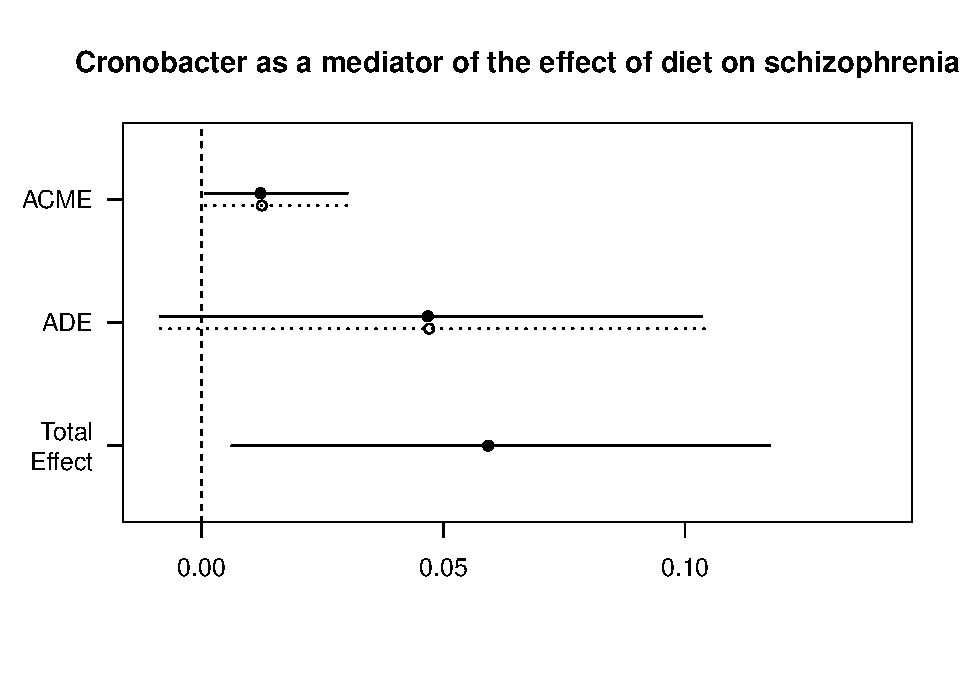
\includegraphics{README_part2_files/figure-latex/plot_crono-1.pdf}

Here, we see that our estimate of the Average Causal Mediation Effect
lies outside of zero. We have partial mediation. In other words, in this
example, it could be the case that part of the effect of diet on
schizophrenia happens because diet also influences \emph{Cronobacter},
which in turn influences schizophrenia.

\newpage

Now, let's take a look at a negative example with \emph{Gordonibacter}.

\hypertarget{code-chunk-gordonibacter-results}{%
\subsubsection{Code chunk: Gordonibacter
results}\label{code-chunk-gordonibacter-results}}

\begin{Shaded}
\begin{Highlighting}[]
\CommentTok{\#Collect the relevant data to display in tables}
\NormalTok{res\_diet.fit2 }\OtherTok{\textless{}{-}} \FunctionTok{coefficients}\NormalTok{(}\FunctionTok{summary}\NormalTok{(diet.fit2))}
\NormalTok{res\_diba.fit2 }\OtherTok{\textless{}{-}} \FunctionTok{coefficients}\NormalTok{(}\FunctionTok{summary}\NormalTok{(diba.fit2))}
\NormalTok{res\_bact.fit2 }\OtherTok{\textless{}{-}} \FunctionTok{coefficients}\NormalTok{(}\FunctionTok{summary}\NormalTok{(bact.fit2))}
\NormalTok{res\_both.fit2 }\OtherTok{\textless{}{-}} \FunctionTok{coefficients}\NormalTok{(}\FunctionTok{summary}\NormalTok{(both.fit2))}
                      
\CommentTok{\#Plot the results in nice looking tables:}
\FunctionTok{kable}\NormalTok{(res\_diet.fit2, }\AttributeTok{digits =} \DecValTok{3}\NormalTok{, }
      \AttributeTok{caption =} \StringTok{"Diet significantly explains phenotype (Estimate of 0.241)."}\NormalTok{)}
\end{Highlighting}
\end{Shaded}

\begin{longtable}[]{@{}lrrrr@{}}
\caption{Diet significantly explains phenotype (Estimate of
0.241).}\tabularnewline
\toprule()
& Estimate & Std. Error & z value &
Pr(\textgreater\textbar z\textbar) \\
\midrule()
\endfirsthead
\toprule()
& Estimate & Std. Error & z value &
Pr(\textgreater\textbar z\textbar) \\
\midrule()
\endhead
(Intercept) & 0.106 & 0.155 & 0.687 & 0.492 \\
diet\_PC1 & 0.241 & 0.122 & 1.972 & 0.049 \\
\bottomrule()
\end{longtable}

\begin{Shaded}
\begin{Highlighting}[]
\FunctionTok{kable}\NormalTok{(res\_diba.fit2, }\AttributeTok{digits =} \DecValTok{3}\NormalTok{, }
      \AttributeTok{caption =} \StringTok{"Diet does not significantly explain Gordonibacter"}\NormalTok{)}
\end{Highlighting}
\end{Shaded}

\begin{longtable}[]{@{}lrrrr@{}}
\caption{Diet does not significantly explain
Gordonibacter}\tabularnewline
\toprule()
& Estimate & Std. Error & t value &
Pr(\textgreater\textbar t\textbar) \\
\midrule()
\endfirsthead
\toprule()
& Estimate & Std. Error & t value &
Pr(\textgreater\textbar t\textbar) \\
\midrule()
\endhead
(Intercept) & -1.734 & 0.114 & -15.175 & 0.000 \\
diet\_PC1 & -0.037 & 0.089 & -0.410 & 0.682 \\
\bottomrule()
\end{longtable}

\begin{Shaded}
\begin{Highlighting}[]
\FunctionTok{kable}\NormalTok{(res\_bact.fit2, }\AttributeTok{digits =} \DecValTok{3}\NormalTok{, }
      \AttributeTok{caption =} \StringTok{"Gordonibacter significantly explains phenotype. This comes as }
\StringTok{      no surprise as saw this in our initial differential abundance analysis."}\NormalTok{)}
\end{Highlighting}
\end{Shaded}

\begin{longtable}[]{@{}lrrrr@{}}
\caption{Gordonibacter significantly explains phenotype. This comes as
no surprise as saw this in our initial differential abundance
analysis.}\tabularnewline
\toprule()
& Estimate & Std. Error & z value &
Pr(\textgreater\textbar z\textbar) \\
\midrule()
\endfirsthead
\toprule()
& Estimate & Std. Error & z value &
Pr(\textgreater\textbar z\textbar) \\
\midrule()
\endhead
(Intercept) & 0.607 & 0.252 & 2.409 & 0.016 \\
Gordonibacter & 0.285 & 0.110 & 2.592 & 0.010 \\
\bottomrule()
\end{longtable}

\begin{Shaded}
\begin{Highlighting}[]
\FunctionTok{kable}\NormalTok{(res\_both.fit2, }\AttributeTok{digits =} \DecValTok{3}\NormalTok{, }
      \AttributeTok{caption =} \StringTok{"In the presence of Gordonibacter, diet explains phenotype even better}
\StringTok{      (Estimate of 0.263)."}\NormalTok{)}
\end{Highlighting}
\end{Shaded}

\begin{longtable}[]{@{}lrrrr@{}}
\caption{In the presence of Gordonibacter, diet explains phenotype even
better (Estimate of 0.263).}\tabularnewline
\toprule()
& Estimate & Std. Error & z value &
Pr(\textgreater\textbar z\textbar) \\
\midrule()
\endfirsthead
\toprule()
& Estimate & Std. Error & z value &
Pr(\textgreater\textbar z\textbar) \\
\midrule()
\endhead
(Intercept) & 0.633 & 0.255 & 2.484 & 0.013 \\
diet\_PC1 & 0.263 & 0.125 & 2.099 & 0.036 \\
Gordonibacter & 0.299 & 0.111 & 2.686 & 0.007 \\
\bottomrule()
\end{longtable}

Looks like we may have a mediation effect here, so let's check out the
results of our mediation analysis: Again, ACME stands for Average Causal
Mediation Effect, whereas ADE stands for Average Direct Effect.

\hypertarget{code-chunk-gordonibacter-mediation-figure}{%
\subsubsection{Code chunk: Gordonibacter mediation
figure}\label{code-chunk-gordonibacter-mediation-figure}}

\begin{Shaded}
\begin{Highlighting}[]
\FunctionTok{summary}\NormalTok{(gordo)}
\end{Highlighting}
\end{Shaded}

\begin{verbatim}
## 
## Causal Mediation Analysis 
## 
## Nonparametric Bootstrap Confidence Intervals with the Percentile Method
## 
##                          Estimate 95% CI Lower 95% CI Upper p-value  
## ACME (control)           -0.00260     -0.01755         0.01   0.720  
## ACME (treated)           -0.00253     -0.01708         0.01   0.720  
## ADE (control)             0.06191      0.00675         0.12   0.038 *
## ADE (treated)             0.06198      0.00675         0.12   0.038 *
## Total Effect              0.05938      0.00130         0.12   0.050 *
## Prop. Mediated (control) -0.04374     -0.67937         0.36   0.758  
## Prop. Mediated (treated) -0.04266     -0.66939         0.36   0.758  
## ACME (average)           -0.00257     -0.01749         0.01   0.720  
## ADE (average)             0.06194      0.00675         0.12   0.038 *
## Prop. Mediated (average) -0.04320     -0.67536         0.36   0.758  
## ---
## Signif. codes:  0 '***' 0.001 '**' 0.01 '*' 0.05 '.' 0.1 ' ' 1
## 
## Sample Size Used: 171 
## 
## 
## Simulations: 1000
\end{verbatim}

\begin{Shaded}
\begin{Highlighting}[]
\CommentTok{\#Let\textquotesingle{}s view the same information in a figure:}
\FunctionTok{plot}\NormalTok{(gordo, }\AttributeTok{main =} \StringTok{"Gordonibacter as a mediator of the effect of diet on schizophrenia"}\NormalTok{)}
\end{Highlighting}
\end{Shaded}

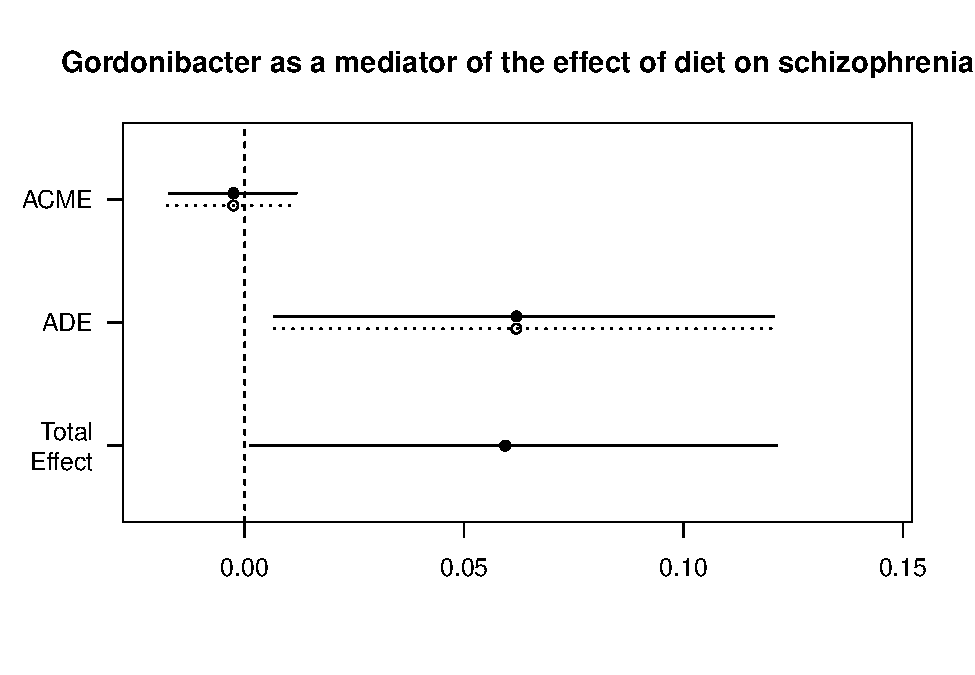
\includegraphics{README_part2_files/figure-latex/plot_gordo-1.pdf}

Here, we see that our estimate of the Average Causal Mediation Effect
lies squarely on zero. No mediation. This makes sense, as diet couldn't
significantly explain the abundance of Gordonibacter.

\begin{center}\rule{0.5\linewidth}{0.5pt}\end{center}

\newpage

\hypertarget{multi-omics-integration}{%
\section{2. Multi-omics integration}\label{multi-omics-integration}}

Here, we will demonstrate how to integrate and subsequently analyse two
'omics data sets. For this, we will use the \texttt{anansi} framework
and package. Studies including both microbiome and metabolomics data are
becoming more common. Often, it would be helpful to integrate both data
sets in order to see if they corroborate each others patterns. All vs
all association is imprecise and likely to yield spurious associations.

The \texttt{anansi} package computes and compares the association
between the features of two 'omics data sets that are known to interact
based on a database such as KEGG. \texttt{anansi} takes a
knowledge-based approach to constrain association search space, only
considering metabolite-function interactions that have been recorded in
a pathway database.

We'll load a complementary training data set using
\texttt{data(FMT\_data)}. This loads a curated snippet from the data set
described in more detail here:
\url{https://doi.org/10.1038/s43587-021-00093-9}\\
A very early version of \texttt{anansi} was used to generate ``Extended
Data Fig. 7'' in that paper.

\hypertarget{code-chunk-load-libraries-and-data}{%
\subsubsection{Code chunk: Load libraries and
data}\label{code-chunk-load-libraries-and-data}}

\begin{Shaded}
\begin{Highlighting}[]
\CommentTok{\#install and load anansi}
\CommentTok{\#devtools::install\_github("thomazbastiaanssen/anansi")}
\FunctionTok{library}\NormalTok{(anansi)}

\CommentTok{\#load ggplot2 and ggforce to plot results}
\FunctionTok{library}\NormalTok{(ggplot2)}
\FunctionTok{library}\NormalTok{(ggforce)}

\CommentTok{\#load dictionary and complementary human{-}readable names for KEGG compounds and orthologues}
\FunctionTok{data}\NormalTok{(dictionary)}
\CommentTok{\#load example data + metadata from FMT Aging study}
\FunctionTok{data}\NormalTok{(FMT\_data)}
\end{Highlighting}
\end{Shaded}

\hypertarget{data-preparation}{%
\subsection{Data preparation}\label{data-preparation}}

The main \texttt{anansi} function expects data in the \texttt{anansiWeb}
format; Basically a list with exactly three tables: The first table,
\texttt{tableY}, should be a count table of metabolites. The second
table, \texttt{tableX}, should be a count table of functions. Both
tables should have columns as features and rows as samples.

The third table should be a binary adjacency matrix with the column
names of \texttt{tableY} as rows and the column names of \texttt{tableX}
as columns. Such an adjacency matrix is provided in the \texttt{anansi}
library and is referred to as a \texttt{dictionary} (because you use it
to look up which metabolites interact with which functions). We can load
it using \texttt{data(dictionary)}.

Though this example uses metabolites and functions, \texttt{anansi} is
able to handle any type of 'omics data, as long as there is a dictionary
available. Because of this, \texttt{anansi} uses the type-naive
nomenclature \texttt{tableY} and \texttt{tableX}. The Y and X refer to
the position these measurements will have in the linear modeling
framework:

\[Y \sim X \times {\text{covariates}}\] \newpage

\hypertarget{a-note-on-functional-microbiome-data}{%
\subsubsection{A note on functional microbiome
data}\label{a-note-on-functional-microbiome-data}}

Two common questions in the host-microbiome field are ``Who's there?''
and ``What are they doing?''.\\
Techniques like 16S sequencing and shotgun metagenomics sequencing are
most commonly used to answer the first question. The second question can
be a bit more tricky - often we'll need functional inference software to
address them. For 16S sequencing, algorithms like \texttt{PICRUSt2} and
\texttt{Piphillin} can be used to infer function. For shotgun
metagenomics, \texttt{HUMANn3} in the bioBakery suite or \texttt{woltka}
can be used.\\
All of these algorithms can produce functional count data in terms of
KEGG Orthologues (KOs). These tables can be directly plugged in to
\texttt{anansi}.

\hypertarget{code-chunk-prepare-data}{%
\subsubsection{Code chunk: Prepare data}\label{code-chunk-prepare-data}}

\begin{Shaded}
\begin{Highlighting}[]
\CommentTok{\#Clean and CLR{-}transform the KEGG orthologue table.}

\CommentTok{\#Only keep functions that are represented in the dictionary.}
\NormalTok{KOs     }\OtherTok{\textless{}{-}}\NormalTok{ FMT\_KOs[}\FunctionTok{row.names}\NormalTok{(FMT\_KOs) }\SpecialCharTok{\%in\%} \FunctionTok{sort}\NormalTok{(}\FunctionTok{unique}\NormalTok{(}\FunctionTok{unlist}\NormalTok{(anansi\_dic))),]}

\CommentTok{\#Cut the decimal part off.}
\NormalTok{KOs     }\OtherTok{\textless{}{-}} \FunctionTok{floor}\NormalTok{(KOs)}

\CommentTok{\#Ensure all entires are numbers.}
\NormalTok{KOs     }\OtherTok{\textless{}{-}} \FunctionTok{apply}\NormalTok{(KOs,}\FunctionTok{c}\NormalTok{(}\DecValTok{1}\NormalTok{,}\DecValTok{2}\NormalTok{),}\ControlFlowTok{function}\NormalTok{(x) }\FunctionTok{as.numeric}\NormalTok{(}\FunctionTok{as.character}\NormalTok{(x)))}

\CommentTok{\#Remove all features with \textless{} 10\% prevalence in the dataset.}
\NormalTok{KOs     }\OtherTok{\textless{}{-}}\NormalTok{ KOs[}\FunctionTok{apply}\NormalTok{(KOs }\SpecialCharTok{==} \DecValTok{0}\NormalTok{, }\DecValTok{1}\NormalTok{, sum) }\SpecialCharTok{\textless{}=}\NormalTok{ (}\FunctionTok{ncol}\NormalTok{(KOs) }\SpecialCharTok{*} \FloatTok{0.90}\NormalTok{), ] }

\CommentTok{\#Perform a centered log{-}ratio transformation on the functional count table.}
\NormalTok{KOs.exp }\OtherTok{\textless{}{-}} \FunctionTok{clr\_c}\NormalTok{(KOs)}

\CommentTok{\#anansi expects samples to be rows and features to be columns. }
\NormalTok{t1      }\OtherTok{\textless{}{-}} \FunctionTok{t}\NormalTok{(FMT\_metab)}
\NormalTok{t2      }\OtherTok{\textless{}{-}} \FunctionTok{t}\NormalTok{(KOs.exp)}
\end{Highlighting}
\end{Shaded}

\hypertarget{weave-a-web}{%
\subsection{Weave a web}\label{weave-a-web}}

The \texttt{weaveWebFromTables()} function can be used to parse the
tables that we prepared above into an \texttt{anansiWeb} object. The
\texttt{anansiWeb} format is a necessary input file for the main
\texttt{anansi} workflow.

\hypertarget{code-chunk-generate-web-object}{%
\subsubsection{Code chunk: Generate web
object}\label{code-chunk-generate-web-object}}

\begin{Shaded}
\begin{Highlighting}[]
\NormalTok{web }\OtherTok{\textless{}{-}} \FunctionTok{weaveWebFromTables}\NormalTok{(}\AttributeTok{tableY =}\NormalTok{ t1, }\AttributeTok{tableX =}\NormalTok{ t2, }\AttributeTok{dictionary =}\NormalTok{ anansi\_dic)}
\end{Highlighting}
\end{Shaded}

\begin{verbatim}
## [1] "Operating in interaction mode"
## [1] "3 were matched between table 1 and the columns of the adjacency matrix"
## [1] "50 were matched between table 2 and the rows of the adjacency matrix"
\end{verbatim}

\newpage

\hypertarget{run-anansi}{%
\subsection{Run anansi}\label{run-anansi}}

The main workspider in this package is called \texttt{anansi}.
Generally, you want to give it three arguments. First, there's
\texttt{web}, which is an \texttt{anansiWeb} object, such as the one we
generated in the above step. Second, there's \texttt{formula}, which
should be a formula. For instance, to assess differential associations
between treatments, we use the formula
\texttt{\textasciitilde{}Treatment}, provided we have a column with that
name in our \texttt{metadata} object, the Third argument.

\hypertarget{code-chunk-run-anansi}{%
\subsubsection{Code chunk: Run anansi}\label{code-chunk-run-anansi}}

\begin{Shaded}
\begin{Highlighting}[]
\NormalTok{anansi\_out }\OtherTok{\textless{}{-}} \FunctionTok{anansi}\NormalTok{(}\AttributeTok{web      =}\NormalTok{ web,          }\CommentTok{\#Generated above}
                     \AttributeTok{method   =} \StringTok{"pearson"}\NormalTok{,    }\CommentTok{\#Define the type of correlation used}
                     \AttributeTok{formula  =} \SpecialCharTok{\textasciitilde{}}\NormalTok{ Legend,     }\CommentTok{\#Compare associations between treatments}
                     \AttributeTok{metadata =}\NormalTok{ FMT\_metadata, }\CommentTok{\#With data referred to in formula as column}
                     \AttributeTok{adjust.method =} \StringTok{"BH"}\NormalTok{,    }\CommentTok{\#Apply the Benjamini{-}Hochberg procedure}
                     \AttributeTok{verbose  =}\NormalTok{ T             }\CommentTok{\#To let you know what\textquotesingle{}s happening}
\NormalTok{                     )}
\end{Highlighting}
\end{Shaded}

\begin{verbatim}
## [1] "Running annotation-based correlations"
## [1] "Running correlations for the following groups: All, Aged yFMT, Aged oFMT, Young yFMT"
## [1] "Fitting models for differential correlation testing"
## [1] "Model type:lm"
## [1] "Adjusting p-values using Benjamini & Hochberg's procedure."
## [1] "Using theoretical distribution."
\end{verbatim}

\hypertarget{spin-to-a-table}{%
\subsection{Spin to a table}\label{spin-to-a-table}}

\texttt{anansi} gives a complex nested \texttt{anansiYarn} object as an
output. Two functions exist that will wrangle your data to more friendly
formats for you. You can either use \texttt{spinToLong()} or
\texttt{spinToWide()}. They will give you long or wide format
data.frames, respectively. For general reporting, we recommend sticking
to the wide format as it's the most legible. You can also use the
\texttt{plot()} method on an \texttt{anansiYarn} object to gain some
insights in the state of your p, q, R and R\textsuperscript{2}
parameters.

\hypertarget{code-chunk-parse-anansi-results}{%
\subsubsection{Code chunk: Parse anansi
results}\label{code-chunk-parse-anansi-results}}

\begin{Shaded}
\begin{Highlighting}[]
\NormalTok{anansiLong }\OtherTok{\textless{}{-}} \FunctionTok{spinToLong}\NormalTok{(}\AttributeTok{anansi\_output =}\NormalTok{ anansi\_out, }\AttributeTok{translate =}\NormalTok{ T, }
                         \AttributeTok{Y\_translation =}\NormalTok{ anansi}\SpecialCharTok{::}\NormalTok{cpd\_translation, }
                         \AttributeTok{X\_translation =}\NormalTok{ anansi}\SpecialCharTok{::}\NormalTok{KO\_translation)  }
\CommentTok{\#Now it\textquotesingle{}s ready to be plugged into ggplot2, though let\textquotesingle{}s clean up a bit more. }

\CommentTok{\#Only consider interactions where the entire model fits well enough. }
\NormalTok{anansiLong }\OtherTok{\textless{}{-}}\NormalTok{ anansiLong[anansiLong}\SpecialCharTok{$}\NormalTok{model\_full\_q.values }\SpecialCharTok{\textless{}} \FloatTok{0.1}\NormalTok{,]}
\end{Highlighting}
\end{Shaded}

\newpage

\hypertarget{plot-the-results}{%
\subsection{Plot the results}\label{plot-the-results}}

The long format can be helpful to plug the data into \texttt{ggplot2}.
Here, we recreate part of the results from the FMT Aging study.

\hypertarget{code-chunk-plot-anansi-results}{%
\subsubsection{Code chunk: Plot anansi
results}\label{code-chunk-plot-anansi-results}}

\begin{Shaded}
\begin{Highlighting}[]
\FunctionTok{ggplot}\NormalTok{(}\AttributeTok{data =}\NormalTok{ anansiLong, }
       \FunctionTok{aes}\NormalTok{(}\AttributeTok{x      =}\NormalTok{ r.values, }
           \AttributeTok{y      =}\NormalTok{ feature\_X, }
           \AttributeTok{fill   =}\NormalTok{ type, }
           \AttributeTok{alpha  =}\NormalTok{ model\_disjointed\_Legend\_p.values }\SpecialCharTok{\textless{}} \FloatTok{0.05}\NormalTok{)) }\SpecialCharTok{+} 
  
  \CommentTok{\#Make a vertical dashed red line at x = 0}
  \FunctionTok{geom\_vline}\NormalTok{(}\AttributeTok{xintercept =} \DecValTok{0}\NormalTok{, }\AttributeTok{linetype =} \StringTok{"dashed"}\NormalTok{, }\AttributeTok{colour =} \StringTok{"red"}\NormalTok{)}\SpecialCharTok{+}
  
  \CommentTok{\#Points show  raw correlation coefficients}
  \FunctionTok{geom\_point}\NormalTok{(}\AttributeTok{shape =} \DecValTok{21}\NormalTok{, }\AttributeTok{size =} \DecValTok{3}\NormalTok{) }\SpecialCharTok{+} 
  
  \CommentTok{\#facet per compound}
\NormalTok{  ggforce}\SpecialCharTok{::}\FunctionTok{facet\_col}\NormalTok{(}\SpecialCharTok{\textasciitilde{}}\NormalTok{feature\_Y, }\AttributeTok{space =} \StringTok{"free"}\NormalTok{, }\AttributeTok{scales =} \StringTok{"free\_y"}\NormalTok{) }\SpecialCharTok{+} 
  
  \CommentTok{\#fix the scales, labels, theme and other layout}
  \FunctionTok{scale\_y\_discrete}\NormalTok{(}\AttributeTok{limits =}\NormalTok{ rev, }\AttributeTok{position =} \StringTok{"right"}\NormalTok{) }\SpecialCharTok{+}
  \FunctionTok{scale\_alpha\_manual}\NormalTok{(}\AttributeTok{values =} \FunctionTok{c}\NormalTok{(}\StringTok{"TRUE"} \OtherTok{=} \DecValTok{1}\NormalTok{, }
                                \StringTok{"FALSE"} \OtherTok{=} \DecValTok{1}\SpecialCharTok{/}\DecValTok{3}\NormalTok{), }\StringTok{"Disjointed association}\SpecialCharTok{\textbackslash{}n}\StringTok{p \textless{} 0.05"}\NormalTok{) }\SpecialCharTok{+}
  \FunctionTok{scale\_fill\_manual}\NormalTok{(}\AttributeTok{values =} \FunctionTok{c}\NormalTok{(}\StringTok{"Young yFMT"} \OtherTok{=} \StringTok{"\#2166ac"}\NormalTok{, }
                               \StringTok{"Aged oFMT"}  \OtherTok{=} \StringTok{"\#b2182b"}\NormalTok{, }
                               \StringTok{"Aged yFMT"}  \OtherTok{=} \StringTok{"\#ef8a62"}\NormalTok{, }
                               \StringTok{"All"}        \OtherTok{=} \StringTok{"gray"}\NormalTok{), }
                    \AttributeTok{breaks =} \FunctionTok{c}\NormalTok{(}\StringTok{"Young yFMT"}\NormalTok{, }\StringTok{"Aged oFMT"}\NormalTok{, }\StringTok{"Aged yFMT"}\NormalTok{, }\StringTok{"All"}\NormalTok{), }
                    \StringTok{"Treatment"}\NormalTok{)}\SpecialCharTok{+}
  \FunctionTok{theme\_bw}\NormalTok{() }\SpecialCharTok{+} 
  \FunctionTok{ylab}\NormalTok{(}\StringTok{""}\NormalTok{) }\SpecialCharTok{+} 
  \FunctionTok{xlab}\NormalTok{(}\StringTok{"Pearson\textquotesingle{}s rho"}\NormalTok{)}
\end{Highlighting}
\end{Shaded}

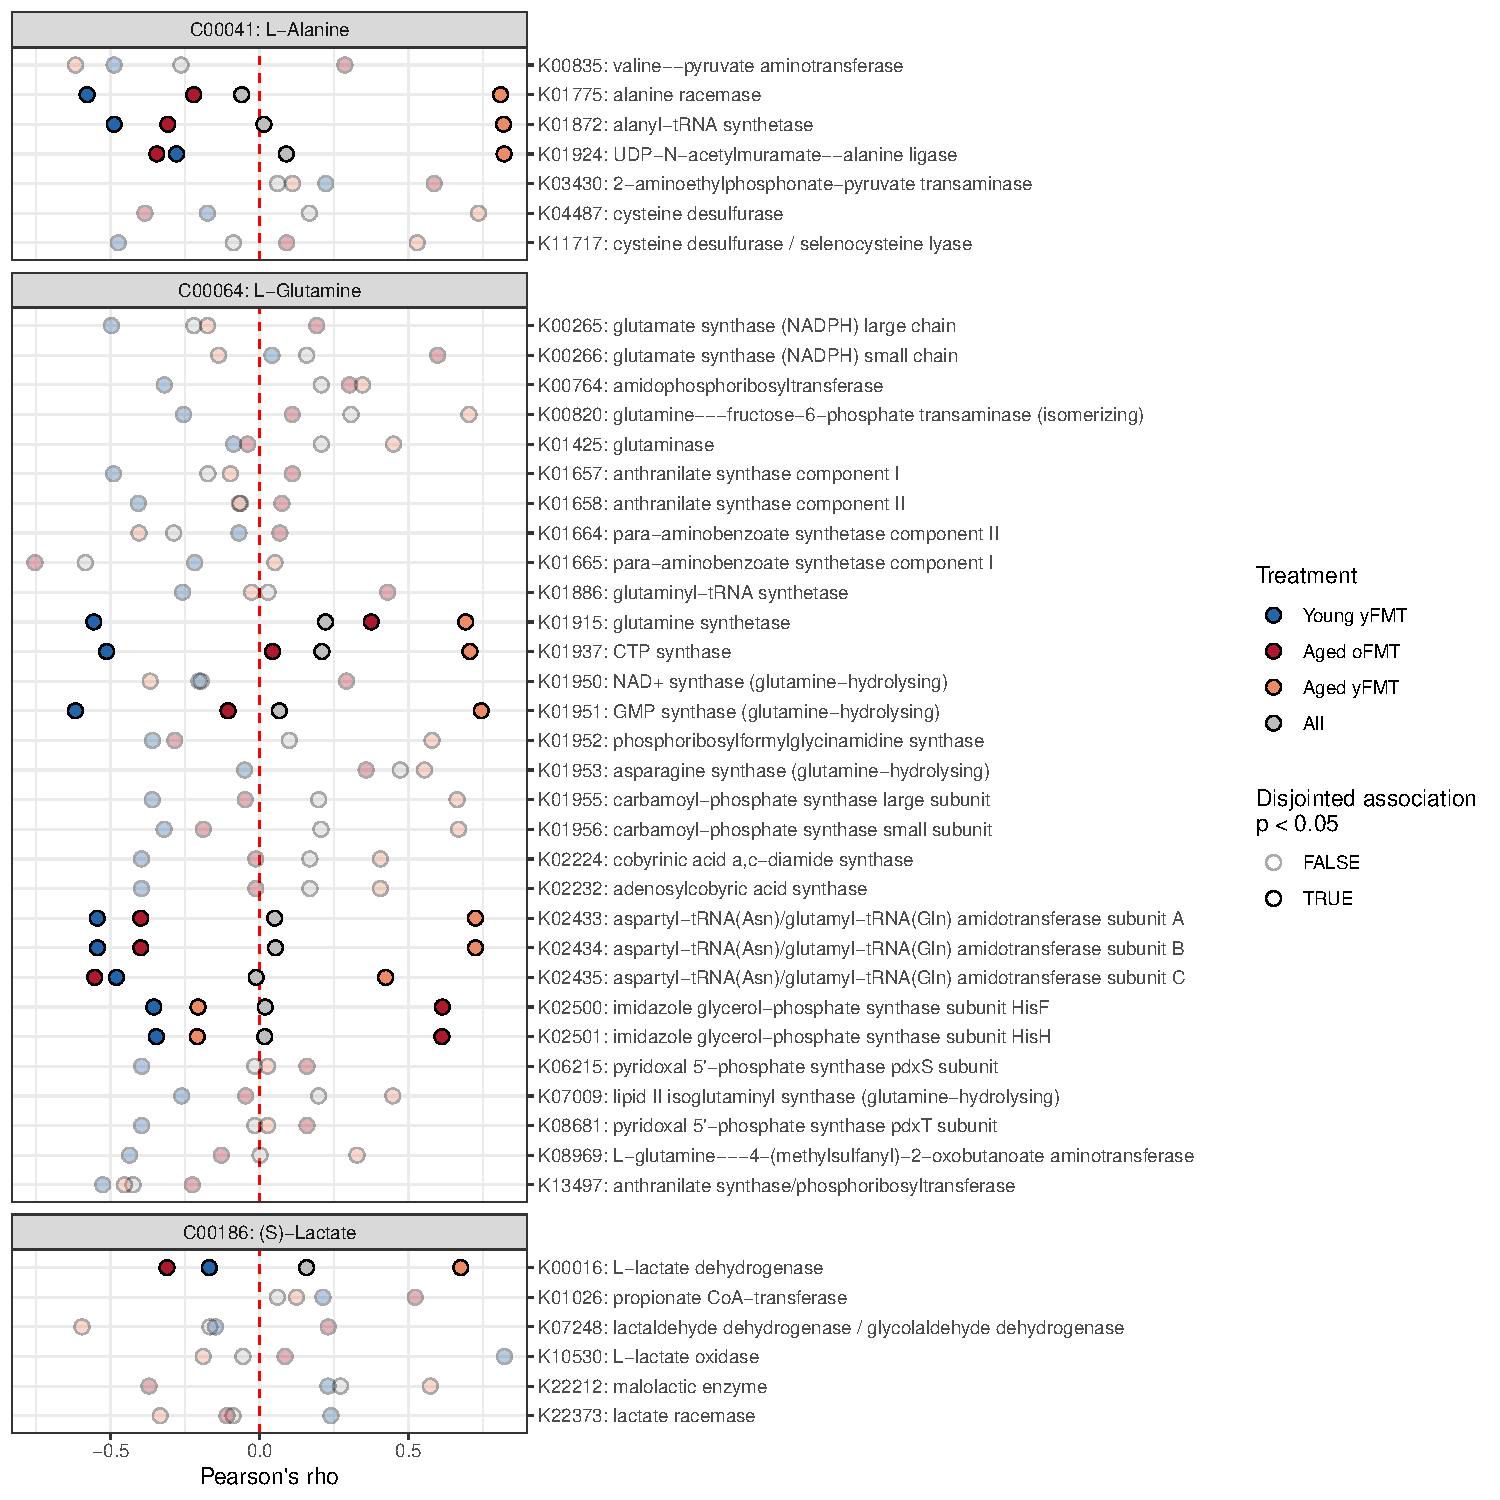
\includegraphics{README_part2_files/figure-latex/plot_FMT-1.pdf}

Here, we can see the per-group correlations between metabolite-function
pairs in terms of Pearson's correlation coefficient on the x-axis.
Opaque points indicate significantly disjointed associations, meaning
that these associations have a significantly different slope between
groups.

\begin{center}\rule{0.5\linewidth}{0.5pt}\end{center}

\newpage

\hypertarget{computing-functional-modules}{%
\section{3. Computing functional
modules}\label{computing-functional-modules}}

Functional modules such as the Gut Brain modules shown here can be a
valuable framework to investigate your data through. One major benefit
of this framework is that you greatly reduce your search-space to
specific functional pathways you're interested in. This will allow you
to greatly save on statistical tests, which in turn will help save
statistical power when accounting for FDR.

Here, we will demonstrate how we got to the Gut Brain modules from our
the schizophrenia data set. Be warned that the first few operations here
are computationally very expensive and should be performed on a server
or similar if possible.

\hypertarget{gathering-and-preparing-our-data-1}{%
\subsection{Gathering and preparing our
data}\label{gathering-and-preparing-our-data-1}}

First, let's download the necessary data from
\texttt{curatedMicrobiomeData}

\hypertarget{code-chunk-download-and-pre-process-microbiome-data}{%
\subsubsection{Code chunk: Download and pre-process microbiome
data}\label{code-chunk-download-and-pre-process-microbiome-data}}

\begin{Shaded}
\begin{Highlighting}[]
\CommentTok{\#Load the relevant libraries}
\FunctionTok{library}\NormalTok{(curatedMetagenomicData)}
\FunctionTok{library}\NormalTok{(SummarizedExperiment)}

\CommentTok{\#Define what data we\textquotesingle{}re interested in. The "|" sign here signifies that we want both.}
\NormalTok{query }\OtherTok{\textless{}{-}} \StringTok{"2021{-}03{-}31.ZhuF\_2020.relative\_abundance|2021{-}03{-}31.ZhuF\_2020.gene\_families"}

\CommentTok{\#Download the specified data. This will take time. }
\NormalTok{ZhuF }\OtherTok{\textless{}{-}} \FunctionTok{curatedMetagenomicData}\NormalTok{(query, }\AttributeTok{counts =}\NormalTok{ T, }\AttributeTok{dryrun =}\NormalTok{ F)}

\CommentTok{\#Extract the relevant data from complex SummarizedExperiment objects}
\NormalTok{Zhu\_F\_gene\_families }\OtherTok{=} \FunctionTok{as.matrix}\NormalTok{( SummarizedExperiment}\SpecialCharTok{::}\FunctionTok{assay}\NormalTok{(ZhuF[[}\DecValTok{1}\NormalTok{]]))     }\CommentTok{\#Functions}
\NormalTok{Zhu\_F\_microbiome    }\OtherTok{=} \FunctionTok{data.frame}\NormalTok{(SummarizedExperiment}\SpecialCharTok{::}\FunctionTok{assay}\NormalTok{(ZhuF[[}\DecValTok{2}\NormalTok{]]))    }\CommentTok{\#Taxa}
\NormalTok{Zhu\_F\_metadata      }\OtherTok{=} \FunctionTok{data.frame}\NormalTok{(SummarizedExperiment}\SpecialCharTok{::}\FunctionTok{colData}\NormalTok{(ZhuF[[}\DecValTok{2}\NormalTok{]]))  }\CommentTok{\#Metadata}

\NormalTok{genus\_lv\_counts }\OtherTok{\textless{}{-}}\NormalTok{ Zhu\_F\_microbiome }\SpecialCharTok{\%\textgreater{}\%} 
  \FunctionTok{rownames\_to\_column}\NormalTok{(}\StringTok{"X"}\NormalTok{) }\SpecialCharTok{\%\textgreater{}\%}
  
  \CommentTok{\#Collapse to genus level}
  \FunctionTok{mutate}\NormalTok{(}\AttributeTok{X =} \FunctionTok{str\_remove}\NormalTok{(X, }\StringTok{"}\SpecialCharTok{\textbackslash{}\textbackslash{}}\StringTok{|s\_\_.*"}\NormalTok{)) }\SpecialCharTok{\%\textgreater{}\%} 
  \FunctionTok{group\_by}\NormalTok{(X) }\SpecialCharTok{\%\textgreater{}\%} 
  \FunctionTok{summarise}\NormalTok{(}\FunctionTok{across}\NormalTok{(}\FunctionTok{everything}\NormalTok{(), sum)) }\SpecialCharTok{\%\textgreater{}\%} 
  \FunctionTok{ungroup}\NormalTok{() }\SpecialCharTok{\%\textgreater{}\%} 
  
  \CommentTok{\#Clean up the names}
  \FunctionTok{mutate}\NormalTok{(}\AttributeTok{X =} \FunctionTok{str\_remove}\NormalTok{(X, }\StringTok{".*}\SpecialCharTok{\textbackslash{}\textbackslash{}}\StringTok{|f\_\_"}\NormalTok{)) }\SpecialCharTok{\%\textgreater{}\%} 
  \FunctionTok{mutate}\NormalTok{(}\AttributeTok{X =} \FunctionTok{str\_replace}\NormalTok{(X, }\StringTok{"}\SpecialCharTok{\textbackslash{}\textbackslash{}}\StringTok{|g\_\_"}\NormalTok{, }\StringTok{"\_"}\NormalTok{)) }\SpecialCharTok{\%\textgreater{}\%} 
  \FunctionTok{mutate}\NormalTok{(}\AttributeTok{X =} \FunctionTok{str\_replace}\NormalTok{(X, }\StringTok{"Clostridiales\_unclassified\_"}\NormalTok{, }\StringTok{"Clostridiales\_"}\NormalTok{)) }\SpecialCharTok{\%\textgreater{}\%} 
  \FunctionTok{filter}\NormalTok{(X }\SpecialCharTok{!=} \StringTok{"Clostridiales\_Clostridiales\_unclassified"}\NormalTok{) }\SpecialCharTok{\%\textgreater{}\%} 
  
  \CommentTok{\#Restore row.names}
  \FunctionTok{column\_to\_rownames}\NormalTok{(}\StringTok{"X"}\NormalTok{)}

\CommentTok{\#Should be identical to file used}
\NormalTok{waldo}\SpecialCharTok{::}\FunctionTok{compare}\NormalTok{(}\FunctionTok{sort}\NormalTok{(}\FunctionTok{row.names}\NormalTok{(genus\_lv\_counts)), }\FunctionTok{sort}\NormalTok{(}\FunctionTok{row.names}\NormalTok{(counts)))}

\CommentTok{\#Now that we have our data, we can write the individual tables to csv files. }
\CommentTok{\#We\textquotesingle{}ll focus on the gene families here, they\textquotesingle{}re necessary to compute Gut Brain modules.}

\FunctionTok{write.csv}\NormalTok{(Zhu\_F\_gene\_families, }\AttributeTok{file =} \StringTok{"uniref90.csv"}\NormalTok{)}
\FunctionTok{write.csv}\NormalTok{(genus\_lv\_counts,     }\AttributeTok{file =} \StringTok{"counts.csv"}\NormalTok{)}
\end{Highlighting}
\end{Shaded}

\hypertarget{convert-to-kegg-orthologues}{%
\subsection{Convert to KEGG
orthologues}\label{convert-to-kegg-orthologues}}

\texttt{Zhu\_F\_gene\_families} contains the functional microbiome in
terms of uniref90. For functional module analysis, we typically want to
get to KEGG orthologues (KOs). Because \texttt{curatedMetagenomicData}
gives essentially biobakery output, we can use commands from the
python-based \texttt{HUMAnN3} pipeline to translate our uniref90 table
to KEGG orthologues. We will not go deeply into this, but see the
excellent documentation here:
\url{https://github.com/biobakery/humann\#humann_regroup_table}

\textbf{The next snippet is not R code, but rather Bash code.}

\hypertarget{code-chunk-convert-functional-table-to-kegg-orthologues}{%
\subsubsection{Code chunk: Convert functional table to KEGG
orthologues}\label{code-chunk-convert-functional-table-to-kegg-orthologues}}

\begin{Shaded}
\begin{Highlighting}[]

\CommentTok{\#First, we may want to change our uniref90 file so that it uses tabs instead of commas}
\FunctionTok{sed} \AttributeTok{{-}E} \StringTok{\textquotesingle{}s/("([\^{}"]*)")?,/\textbackslash{}2\textbackslash{}t/g\textquotesingle{}}\NormalTok{ uniref90.csv  }\OperatorTok{\textgreater{}}\NormalTok{ uniref90.tsv}

\CommentTok{\#Then, let\textquotesingle{}s use humann\_regroup\_table from HUMAnN3 to convert to KEGG orthologues:}
\ExtensionTok{humann\_regroup\_table} \AttributeTok{{-}i}\NormalTok{ uniref90.tsv }\AttributeTok{{-}g}\NormalTok{ uniref90\_ko }\AttributeTok{{-}o}\NormalTok{ guidebook\_out\_KOs.tsv}
\end{Highlighting}
\end{Shaded}

\newpage

\hypertarget{compute-functional-modules}{%
\subsection{Compute functional
modules}\label{compute-functional-modules}}

Now that we have our functional microbiome in terms of KEGG orthologues,
we can load them back into R. An added benefit is that the KEGG
orthologues table is much smaller than the uniref90 table, so we can
deal with it on our computer locally if we so choose. In order to do
this, we will require the \texttt{omixer-rpmR} library which can be
found of github. If you're working with functional inference data from a
16S experiment, such as output from \texttt{PICRUSt2}, you should be
able to read the table in and compute functional modules starting at
this step. The file you're looking for would be called something like
\texttt{pred\_metagenome\_unstrat.tsv} in that case.

\hypertarget{code-chunk-generate-functional-modules}{%
\subsubsection{Code chunk: Generate functional
modules}\label{code-chunk-generate-functional-modules}}

\begin{Shaded}
\begin{Highlighting}[]
\CommentTok{\#Load the required package}
\FunctionTok{library}\NormalTok{(omixerRpm) }\CommentTok{\#devtools::install\_github("omixer/omixer{-}rpmR")}

\CommentTok{\#Load the KEGG orthologue table into R. }
\CommentTok{\#Note that KEGG orthologue names should be the in first column, not the row names.  }
\NormalTok{KOs }\OtherTok{\textless{}{-}} \FunctionTok{read.delim}\NormalTok{(}\StringTok{"guidebook\_out\_KOs.tsv"}\NormalTok{, }\AttributeTok{header =}\NormalTok{ T)}

\CommentTok{\#listDB will tell you which databases are available to annotate the functional data with. }
\FunctionTok{listDB}\NormalTok{()}

\CommentTok{\#Pick the most recent GBM database}
\NormalTok{db }\OtherTok{\textless{}{-}} \FunctionTok{loadDB}\NormalTok{(}\AttributeTok{name =} \StringTok{"GBMs.v1.0"}\NormalTok{)}

\CommentTok{\#Calculate GBM abundance and convert the output to a nice data.frame}
\NormalTok{GBMs }\OtherTok{\textless{}{-}} \FunctionTok{rpm}\NormalTok{(}\AttributeTok{x =}\NormalTok{ KOs,  }\AttributeTok{module.db =}\NormalTok{ db)}
\NormalTok{GBMs }\OtherTok{\textless{}{-}} \FunctionTok{asDataFrame}\NormalTok{(GBMs, }\StringTok{"abundance"}\NormalTok{)}

\CommentTok{\#Write the file to a csv to save it. }
\FunctionTok{write.csv}\NormalTok{(GBMs, }\AttributeTok{file =} \StringTok{"GBMs\_guidebook.csv"}\NormalTok{)}

\CommentTok{\#While we\textquotesingle{}re at it, let\textquotesingle{}s do GMMs too: First check the names of the available databases:}
\FunctionTok{listDB}\NormalTok{()}

\CommentTok{\#Pick the most recent GMM database}
\NormalTok{db }\OtherTok{\textless{}{-}} \FunctionTok{loadDB}\NormalTok{(}\AttributeTok{name =} \StringTok{"GMMs.v1.07"}\NormalTok{)}

\CommentTok{\#Calculate GMM abundance and convert the output to a nice data.frame}
\NormalTok{GMMs }\OtherTok{\textless{}{-}} \FunctionTok{rpm}\NormalTok{(}\AttributeTok{x =}\NormalTok{ KOs,  }\AttributeTok{module.db =}\NormalTok{ db)}
\NormalTok{GMMs }\OtherTok{\textless{}{-}} \FunctionTok{asDataFrame}\NormalTok{(GMMs, }\StringTok{"abundance"}\NormalTok{)}

\CommentTok{\#Write the file to a csv to save it. }
\FunctionTok{write.csv}\NormalTok{(GMMs, }\AttributeTok{file =} \StringTok{"GMMs\_guidebook.csv"}\NormalTok{)}
\end{Highlighting}
\end{Shaded}

And the resulting files are ready for statistical analysis! I would like
to note here that it's also possible to perform a stratified functional
module analysis, where the contribution of each taxon to each functional
module is also considered. However, this explosively increases the
dimensionality of your data (i.e.~you get way more rows in our case). I
would only recommend doing this as a targeted analysis as the power of
any statistical tests will suffer greatly and the results will be almost
impossible to interpret.

\begin{center}\rule{0.5\linewidth}{0.5pt}\end{center}

\newpage

\hypertarget{volatility-analysis}{%
\section{4. Volatility Analysis}\label{volatility-analysis}}

Volatility refers to the degree of instability (or change over time) in
the microbiome. High volatility, i.e.~an unstable microbiome, has been
associated with an exaggerated stress response and conditions like IBS.
Here, we'll demonstrate how one would go about calculating volatility in
a real data set. Volatility analysis requires at least two time points
per sample. Because of this, we cannot use the schizophrenia data set
which only features single snapshots of the microbiome.

We'll be taking a look at the datasets used in the original Volatility
paper: \emph{Volatility as a Concept to Understand the Impact of Stress
on the Microbiome} (DOI: 10.1016/j.psyneuen.2020.105047). Very briefly,
mice were separated into two groups: Control and Stress. Faecal samples
were taken twice, with a 10-day period in between. In this 10-day
period, the mice in the Stress group were subjected to daily social
defeat stress, whereas the Control mice were left alone. When we
compared the degree of change in the microbiome (i.e.~Volatility)
between the two groups of mice, the Stressed mice consistently displayed
higher levels of volatility than the control mice. Our reviewers asked
us to replicate the experiment and we did so. The two cohorts are
labeled discovery and validation. This data has been included in the
\texttt{volatility} library on github for easy access purposes.

Traditionally, microbiome studies featuring high-throughput sequencing
data only consider a single time point. However, there is utility in
considering microbiomes as dynamic microbial ecosystems that change over
time. By measuring the microbiome longitudinally and computing
volatility, additional information can be revealed that would otherwise
be missed. For instance, in the original volatility study, we found that
volatility after stress is positively associated with severity of the
stress response, including in terms of behaviour and
hypothalamic-pituitary-adrenal (HPA) axis activity, both in mice and in
humans.

\hypertarget{setup}{%
\subsection{Setup}\label{setup}}

OK, now let's get started.

\hypertarget{code-chunk-load-data}{%
\subsubsection{Code chunk: Load data}\label{code-chunk-load-data}}

\begin{Shaded}
\begin{Highlighting}[]
\CommentTok{\#Install and load volatility library}
\FunctionTok{library}\NormalTok{(volatility)     }\CommentTok{\#devtools::install\_github("thomazbastiaanssen/volatility")}

\CommentTok{\#Load tidyverse to wrangle and plot results.}
\FunctionTok{library}\NormalTok{(tidyverse)}

\CommentTok{\#Load example data + metadata from the volatility study.}
\FunctionTok{data}\NormalTok{(volatility\_data)}
\end{Highlighting}
\end{Shaded}

\newpage

\hypertarget{considering-our-input-data}{%
\subsection{Considering our input
data}\label{considering-our-input-data}}

The main \texttt{volatility} function does all the heavy lifting here.
It expects two arguments: The first argument is \texttt{counts}, a
microbiome feature count table, with columns as samples and rows and
features. The \texttt{vola\_genus\_table} object is an example of an
appropriately formatted count table.

\hypertarget{code-chunk-examine-required-data-format}{%
\subsubsection{Code chunk: Examine required data
format}\label{code-chunk-examine-required-data-format}}

\begin{Shaded}
\begin{Highlighting}[]
\NormalTok{vola\_genus\_table[}\DecValTok{4}\SpecialCharTok{:}\DecValTok{9}\NormalTok{,}\DecValTok{1}\SpecialCharTok{:}\DecValTok{2}\NormalTok{]}
\end{Highlighting}
\end{Shaded}

\begin{verbatim}
##                               Validation_Pre_Control_1 Validation_Pre_Control_2
## Atopobiaceae_Olsenella                               0                        0
## Coriobacteriaceae_Collinsella                        0                        0
## Eggerthellaceae_DNF00809                           102                       47
## Eggerthellaceae_Enterorhabdus                       53                      114
## Eggerthellaceae_Parvibacter                         21                       20
## Bacteroidaceae_Bacteroides                         616                      453
\end{verbatim}

The second arguent is \texttt{metadata}, a vector in the same order as
the count table, denoting which samples are from the same source. The
column \texttt{ID} in \texttt{vola\_metadata} is appropriate for this.

\hypertarget{code-chunk-examine-required-metadata-format}{%
\subsubsection{Code chunk: Examine required metadata
format}\label{code-chunk-examine-required-metadata-format}}

\begin{Shaded}
\begin{Highlighting}[]
\FunctionTok{head}\NormalTok{(vola\_metadata, }\DecValTok{5}\NormalTok{)}
\end{Highlighting}
\end{Shaded}

\begin{verbatim}
##                  sample_ID     cohort timepoint treatment ID
## 1 Validation_Pre_Control_1 Validation       Pre   Control  1
## 2 Validation_Pre_Control_2 Validation       Pre   Control  2
## 3 Validation_Pre_Control_3 Validation       Pre   Control  3
## 4 Validation_Pre_Control_4 Validation       Pre   Control  4
## 5 Validation_Pre_Control_5 Validation       Pre   Control  5
\end{verbatim}

\hypertarget{code-chunk-prepare-the-data-for-plotting}{%
\subsubsection{Code chunk: Prepare the data for
plotting}\label{code-chunk-prepare-the-data-for-plotting}}

\begin{Shaded}
\begin{Highlighting}[]
\CommentTok{\#This part should feel very reminiscent of what we did in chapters 1 \& 3. }
\NormalTok{counts  }\OtherTok{\textless{}{-}}\NormalTok{ vola\_genus\_table[,vola\_metadata}\SpecialCharTok{$}\NormalTok{sample\_ID]}

\CommentTok{\#Fork off your count data so that you always have an untouched version handy.}
\NormalTok{genus   }\OtherTok{\textless{}{-}}\NormalTok{ counts}

\CommentTok{\#make sure our count data is all numbers}
\NormalTok{genus   }\OtherTok{\textless{}{-}} \FunctionTok{apply}\NormalTok{(genus,}\FunctionTok{c}\NormalTok{(}\DecValTok{1}\NormalTok{,}\DecValTok{2}\NormalTok{),}\ControlFlowTok{function}\NormalTok{(x) }\FunctionTok{as.numeric}\NormalTok{(}\FunctionTok{as.character}\NormalTok{(x)))}

\CommentTok{\#Remove features with prevalence \textless{} 10\% in two steps:}
\CommentTok{\#First, determine how often every feature is absent in a sample}
\NormalTok{n\_zeroes }\OtherTok{\textless{}{-}} \FunctionTok{rowSums}\NormalTok{(genus }\SpecialCharTok{==} \DecValTok{0}\NormalTok{)}

\CommentTok{\#Then, remove features that are absent in more than your threshold (90\% in this case).}
\NormalTok{genus    }\OtherTok{\textless{}{-}}\NormalTok{ genus[n\_zeroes }\SpecialCharTok{\textless{}=} \FunctionTok{round}\NormalTok{(}\FunctionTok{ncol}\NormalTok{(genus) }\SpecialCharTok{*} \FloatTok{0.90}\NormalTok{),]}

\CommentTok{\#Perform a CLR transformation}
\NormalTok{genus.exp }\OtherTok{\textless{}{-}} \FunctionTok{clr\_c}\NormalTok{(genus)}

\CommentTok{\#Apply the base R principal component analysis function on our CLR{-}transformed data.}
\NormalTok{data.a.pca  }\OtherTok{\textless{}{-}} \FunctionTok{prcomp}\NormalTok{(}\FunctionTok{t}\NormalTok{(genus.exp))}
\end{Highlighting}
\end{Shaded}

\newpage

\hypertarget{plot-data}{%
\subsection{Plot data}\label{plot-data}}

\hypertarget{code-chunk-plot-longitudinal-pca}{%
\subsubsection{Code chunk: Plot longitudinal
PCA}\label{code-chunk-plot-longitudinal-pca}}

\begin{Shaded}
\begin{Highlighting}[]
\CommentTok{\#Extract the amount of variance the first four components explain for plotting. }
\NormalTok{pc1 }\OtherTok{\textless{}{-}} \FunctionTok{round}\NormalTok{(data.a.pca}\SpecialCharTok{$}\NormalTok{sdev[}\DecValTok{1}\NormalTok{]}\SpecialCharTok{\^{}}\DecValTok{2}\SpecialCharTok{/}\FunctionTok{sum}\NormalTok{(data.a.pca}\SpecialCharTok{$}\NormalTok{sdev}\SpecialCharTok{\^{}}\DecValTok{2}\NormalTok{),}\DecValTok{4}\NormalTok{) }\SpecialCharTok{*} \DecValTok{100}
\NormalTok{pc2 }\OtherTok{\textless{}{-}} \FunctionTok{round}\NormalTok{(data.a.pca}\SpecialCharTok{$}\NormalTok{sdev[}\DecValTok{2}\NormalTok{]}\SpecialCharTok{\^{}}\DecValTok{2}\SpecialCharTok{/}\FunctionTok{sum}\NormalTok{(data.a.pca}\SpecialCharTok{$}\NormalTok{sdev}\SpecialCharTok{\^{}}\DecValTok{2}\NormalTok{),}\DecValTok{4}\NormalTok{) }\SpecialCharTok{*} \DecValTok{100}
\NormalTok{pc3 }\OtherTok{\textless{}{-}} \FunctionTok{round}\NormalTok{(data.a.pca}\SpecialCharTok{$}\NormalTok{sdev[}\DecValTok{3}\NormalTok{]}\SpecialCharTok{\^{}}\DecValTok{2}\SpecialCharTok{/}\FunctionTok{sum}\NormalTok{(data.a.pca}\SpecialCharTok{$}\NormalTok{sdev}\SpecialCharTok{\^{}}\DecValTok{2}\NormalTok{),}\DecValTok{4}\NormalTok{) }\SpecialCharTok{*} \DecValTok{100}
\NormalTok{pc4 }\OtherTok{\textless{}{-}} \FunctionTok{round}\NormalTok{(data.a.pca}\SpecialCharTok{$}\NormalTok{sdev[}\DecValTok{4}\NormalTok{]}\SpecialCharTok{\^{}}\DecValTok{2}\SpecialCharTok{/}\FunctionTok{sum}\NormalTok{(data.a.pca}\SpecialCharTok{$}\NormalTok{sdev}\SpecialCharTok{\^{}}\DecValTok{2}\NormalTok{),}\DecValTok{4}\NormalTok{) }\SpecialCharTok{*} \DecValTok{100}

\CommentTok{\#Extract the scores for every sample for the first four components for plotting. }
\NormalTok{pca  }\OtherTok{=} \FunctionTok{data.frame}\NormalTok{(}\AttributeTok{PC1 =}\NormalTok{ data.a.pca}\SpecialCharTok{$}\NormalTok{x[,}\DecValTok{1}\NormalTok{], }
                  \AttributeTok{PC2 =}\NormalTok{ data.a.pca}\SpecialCharTok{$}\NormalTok{x[,}\DecValTok{2}\NormalTok{], }
                  \AttributeTok{PC3 =}\NormalTok{ data.a.pca}\SpecialCharTok{$}\NormalTok{x[,}\DecValTok{3}\NormalTok{], }
                  \AttributeTok{PC4 =}\NormalTok{ data.a.pca}\SpecialCharTok{$}\NormalTok{x[,}\DecValTok{4}\NormalTok{])}

\CommentTok{\#Add relevant information from the metadata. }
\CommentTok{\#Note that ID here refers to the mouse ID, not the sample ID. }
\NormalTok{pca}\SpecialCharTok{$}\NormalTok{ID                  }\OtherTok{=}\NormalTok{ vola\_metadata}\SpecialCharTok{$}\NormalTok{ID}
\NormalTok{pca}\SpecialCharTok{$}\NormalTok{Legend              }\OtherTok{=}\NormalTok{ vola\_metadata}\SpecialCharTok{$}\NormalTok{treatment}
\NormalTok{pca}\SpecialCharTok{$}\NormalTok{Timepoint           }\OtherTok{=}\NormalTok{ vola\_metadata}\SpecialCharTok{$}\NormalTok{timepoint}
\NormalTok{pca}\SpecialCharTok{$}\NormalTok{Cohort              }\OtherTok{=}\NormalTok{ vola\_metadata}\SpecialCharTok{$}\NormalTok{cohort}

\CommentTok{\#Plot the first two components of the PCA.}
\FunctionTok{ggplot}\NormalTok{(pca, }\FunctionTok{aes}\NormalTok{(}\AttributeTok{x       =}\NormalTok{ PC1, }
                \AttributeTok{y       =}\NormalTok{ PC2, }
                \AttributeTok{fill    =}\NormalTok{ Legend,}
                \AttributeTok{colour  =}\NormalTok{ Legend,}
                \AttributeTok{shape   =}\NormalTok{ Timepoint, }
                \AttributeTok{group   =}\NormalTok{ ID)) }\SpecialCharTok{+}  
  \CommentTok{\#Add a line first, it will link points that share an ID. }
  \FunctionTok{geom\_line}\NormalTok{() }\SpecialCharTok{+}
  
  \CommentTok{\#Then add the points.}
  \FunctionTok{geom\_point}\NormalTok{(}\AttributeTok{size =} \DecValTok{3}\NormalTok{, }\AttributeTok{col =} \StringTok{"black"}\NormalTok{) }\SpecialCharTok{+} 
  
  \CommentTok{\#Plot the two cohorts separately. }
  \FunctionTok{facet\_wrap}\NormalTok{(}\SpecialCharTok{\textasciitilde{}}\NormalTok{Cohort, }\AttributeTok{scales =} \StringTok{"free\_x"}\NormalTok{, }\AttributeTok{strip.position =} \StringTok{"top"}\NormalTok{) }\SpecialCharTok{+}
  
  \CommentTok{\#Improve appearance.}
  \FunctionTok{scale\_fill\_manual}\NormalTok{(  }\AttributeTok{values =} \FunctionTok{c}\NormalTok{(}\StringTok{"Control"}  \OtherTok{=} \StringTok{"\#1f78b4"}\NormalTok{, }
                                 \StringTok{"Stress"}   \OtherTok{=} \StringTok{"\#e31a1c"}\NormalTok{)) }\SpecialCharTok{+} 
  \FunctionTok{scale\_colour\_manual}\NormalTok{(}\AttributeTok{values =} \FunctionTok{c}\NormalTok{(}\StringTok{"Control"}  \OtherTok{=} \StringTok{"\#3690c0"}\NormalTok{, }
                                 \StringTok{"Stress"}   \OtherTok{=} \StringTok{"\#cb181d"}\NormalTok{)) }\SpecialCharTok{+} 
  \FunctionTok{scale\_shape\_manual}\NormalTok{( }\AttributeTok{values =} \FunctionTok{c}\NormalTok{(}\StringTok{"Pre"}  \OtherTok{=} \DecValTok{21}\NormalTok{, }
                                \StringTok{"Post"} \OtherTok{=} \DecValTok{24}\NormalTok{)) }\SpecialCharTok{+}  
  \FunctionTok{theme\_bw}\NormalTok{() }\SpecialCharTok{+}
  \FunctionTok{xlab}\NormalTok{(}\FunctionTok{paste}\NormalTok{(}\StringTok{"PC1: "}\NormalTok{, pc1,  }\StringTok{"\%"}\NormalTok{, }\AttributeTok{sep=}\StringTok{""}\NormalTok{)) }\SpecialCharTok{+} 
  \FunctionTok{ylab}\NormalTok{(}\FunctionTok{paste}\NormalTok{(}\StringTok{"PC2: "}\NormalTok{, pc2,  }\StringTok{"\%"}\NormalTok{, }\AttributeTok{sep=}\StringTok{""}\NormalTok{)) }\SpecialCharTok{+} 
  \FunctionTok{theme}\NormalTok{(}\AttributeTok{text =} \FunctionTok{element\_text}\NormalTok{(}\AttributeTok{size =} \DecValTok{12}\NormalTok{)) }\SpecialCharTok{+}
  \FunctionTok{guides}\NormalTok{(}\AttributeTok{fill =} \FunctionTok{guide\_legend}\NormalTok{(}\AttributeTok{override.aes =} \FunctionTok{list}\NormalTok{(}\AttributeTok{shape =} \DecValTok{22}\NormalTok{)))}
\end{Highlighting}
\end{Shaded}

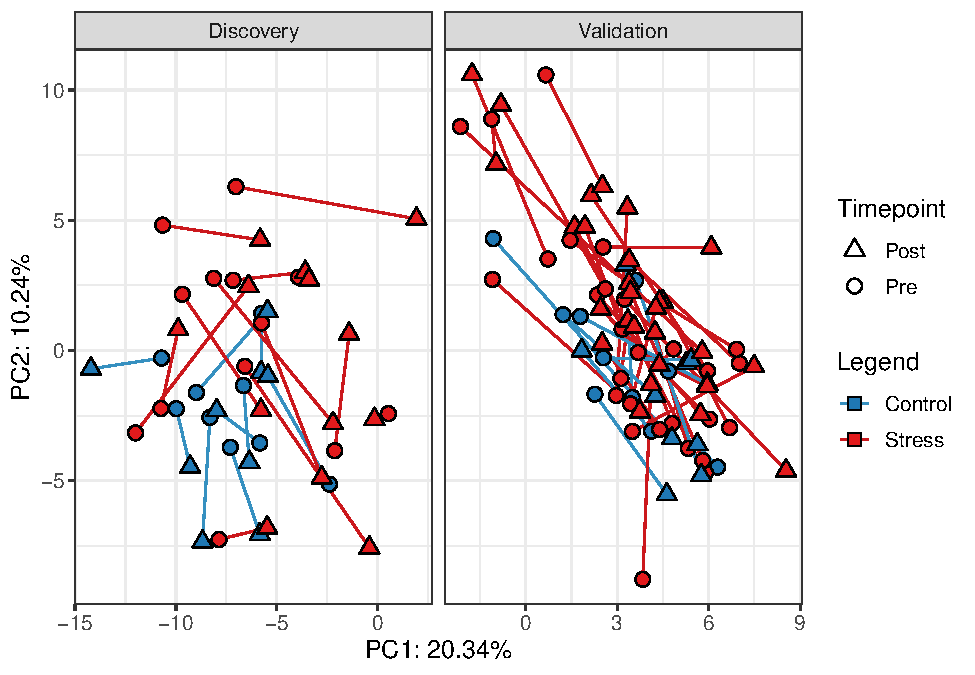
\includegraphics{README_part2_files/figure-latex/unnamed-chunk-12-1.pdf}

We can see that points from the same mouse are connected by a line. It
looks like some lines are longer than others, implying that some
microbiomes have changed more than others over the 10 days. However,
We're only looking at about 30\% of the variance here, so it's hard to
say anything conclusive.

\hypertarget{compute-volatility}{%
\subsection{Compute volatility}\label{compute-volatility}}

Volatility between two samples can be easily calculated using the
titular \texttt{volatilty} function in the library by the same name.
Under the hood, volatility can be calculated as the euclidean distance
over CLR-transformed count data.

\hypertarget{code-chunk-calculate-volatility}{%
\subsubsection{Code chunk: Calculate
volatility}\label{code-chunk-calculate-volatility}}

\begin{Shaded}
\begin{Highlighting}[]
\NormalTok{vola\_out }\OtherTok{\textless{}{-}} \FunctionTok{volatility}\NormalTok{(}\AttributeTok{counts =}\NormalTok{ genus, }\AttributeTok{metadata =}\NormalTok{ vola\_metadata}\SpecialCharTok{$}\NormalTok{ID)}

\FunctionTok{head}\NormalTok{(vola\_out)}
\end{Highlighting}
\end{Shaded}

\begin{verbatim}
##   ID volatility
## 1  1  13.275363
## 2 10  12.979717
## 3 11  15.987468
## 4 13  14.902772
## 5 14   8.094823
## 6 15   9.506299
\end{verbatim}

The output of the main \texttt{volatility} function is a data.frame with
two columns. \texttt{ID} corresponds to the pairs of samples passed on
in the \texttt{metadata} argument, whereas \texttt{volatility} shows the
measured volatility between those samples in terms of Aitchison distance
(Euclidean distance of CLR-transformed counts).

\newpage

\hypertarget{plot-the-results-1}{%
\subsection{Plot the results}\label{plot-the-results-1}}

\hypertarget{code-chunk-plot-volatility}{%
\subsubsection{Code chunk: Plot
volatility}\label{code-chunk-plot-volatility}}

\begin{Shaded}
\begin{Highlighting}[]
\NormalTok{vola\_out }\SpecialCharTok{\%\textgreater{}\%}
  \CommentTok{\#Merge the volatilty output with the rest of the metadata using the shared "ID" column.}
  \FunctionTok{left\_join}\NormalTok{(vola\_metadata[vola\_metadata}\SpecialCharTok{$}\NormalTok{timepoint }\SpecialCharTok{==} \StringTok{"Pre"}\NormalTok{,], }\StringTok{"ID"}\NormalTok{) }\SpecialCharTok{\%\textgreater{}\%}
  
  \CommentTok{\#Pipe into ggplot.}
  \FunctionTok{ggplot}\NormalTok{(}\FunctionTok{aes}\NormalTok{(}\AttributeTok{x =}\NormalTok{ treatment, }\AttributeTok{y =}\NormalTok{ volatility, }\AttributeTok{fill =}\NormalTok{ treatment)) }\SpecialCharTok{+}
  
  \CommentTok{\#Define geoms, boxplots overlayed with data points in this case.}
  \FunctionTok{geom\_boxplot}\NormalTok{(}\AttributeTok{alpha =} \DecValTok{1}\SpecialCharTok{/}\DecValTok{2}\NormalTok{, }\AttributeTok{coef =} \DecValTok{10}\NormalTok{)}\SpecialCharTok{+}
  \FunctionTok{geom\_point}\NormalTok{(}\AttributeTok{shape =} \DecValTok{21}\NormalTok{) }\SpecialCharTok{+}
  
  \CommentTok{\#Split the plot by cohort.}
  \FunctionTok{facet\_wrap}\NormalTok{(}\SpecialCharTok{\textasciitilde{}}\NormalTok{cohort) }\SpecialCharTok{+}
  
  \CommentTok{\#Tweak appearance.}
  \FunctionTok{scale\_fill\_manual}\NormalTok{(}\AttributeTok{values =} \FunctionTok{c}\NormalTok{(}\StringTok{"Control"} \OtherTok{=} \StringTok{"\#3690c0"}\NormalTok{, }\StringTok{"Stress"}  \OtherTok{=} \StringTok{"\#cb181d"}\NormalTok{)) }\SpecialCharTok{+}
  \FunctionTok{theme\_bw}\NormalTok{() }\SpecialCharTok{+}
  \FunctionTok{xlab}\NormalTok{(}\StringTok{""}\NormalTok{) }\SpecialCharTok{+}
  \FunctionTok{ylab}\NormalTok{(}\StringTok{"Volatility (Aitchison distance)"}\NormalTok{)}
\end{Highlighting}
\end{Shaded}

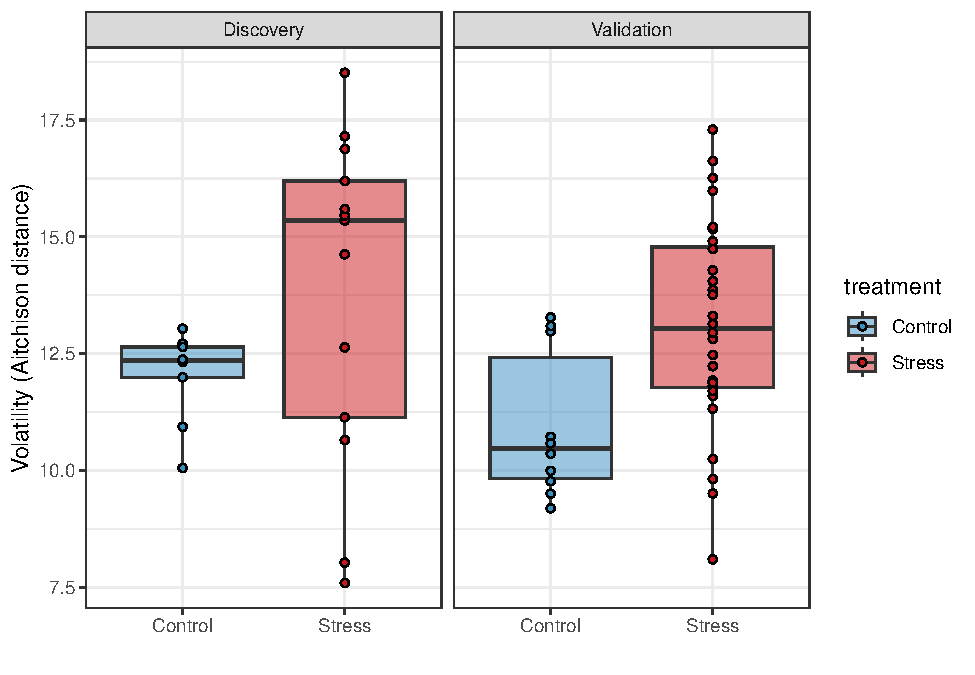
\includegraphics{README_part2_files/figure-latex/plot_volatility-1.pdf}

\begin{center}\rule{0.5\linewidth}{0.5pt}\end{center}

\newpage

\hypertarget{discussion}{%
\section{5. Discussion}\label{discussion}}

Here, we have presented four separate primers for techniques from four
distinct topics, namely causal inference, multi-omics integration,
mesoscale analysis and temporal analysis, and how one may go about
applying them to microbiome-gut-brain axis experiments. While these
techniques and corresponding fields may seem unrelated, we are of the
opinion that all four will be essential to move the microbiome-gut-brain
axis field forward towards an ecology oriented, mechanistic
understanding.

As said in the discussion of part 1 of this perspective, this document
is just a template. Depending on the experimental setup, findings and
experimental questions, you may want to choose a differing approach.
Given the highly complex nature of microbiome data, one should ideally
avoid blindly applying models and pipelines without understanding what
they are doing. D.R. Cox is famously ascribed the statement:
\emph{``Most real life statistical problems have one or more nonstandard
features. There are no routine statistical questions; only questionable
statistical routines.''} We find this holds true for the microbiome as
well, even more so for these more advanced techniques than for the ones
presented in part 1 of this perspective piece. In particular, it is
crucial that we apply our biological knowledge to determine how exactly
to use these techniques. For instance, when performing a mediation
analysis in section 1, it is crucial to have a biological reason why one
would expect the effect of a variable on an outcome to be moderated by a
second variable. Similarly, with the multi-omics integration using
anansi in section 2, we're relying on pre-existing biological knowledge
in the form of the KEGG database to only investigate interactions
between metabolites and enzymatic functions that could take place,
rather than naively assessing all of them.

Clear communication, both in terms of describing and explaining our
methods as well as in terms of figure presentation, are essential for
the health of the field. Indeed, failing to do so can lead to confusion
among our peers. We hope that both aspiring and veteran
bioinformaticians will find our guide helpful. We have tried to model
this piece after what we would have loved to have access to ourselves
when we first set out to study the microbiome.

\begin{center}\rule{0.5\linewidth}{0.5pt}\end{center}

\newpage

\hypertarget{session-info}{%
\section{Session Info}\label{session-info}}

\begin{Shaded}
\begin{Highlighting}[]
\NormalTok{sessioninfo}\SpecialCharTok{::}\FunctionTok{session\_info}\NormalTok{()}
\end{Highlighting}
\end{Shaded}

\begin{verbatim}
## - Session info ---------------------------------------------------------------
##  setting  value
##  version  R version 4.2.2 Patched (2022-11-10 r83330)
##  os       Ubuntu 18.04.6 LTS
##  system   x86_64, linux-gnu
##  ui       X11
##  language en_IE:en
##  collate  en_IE.UTF-8
##  ctype    en_IE.UTF-8
##  tz       Europe/Dublin
##  date     2023-08-21
##  pandoc   2.19.2 @ /usr/lib/rstudio/resources/app/bin/quarto/bin/tools/ (via rmarkdown)
## 
## - Packages -------------------------------------------------------------------
##  package       * version    date (UTC) lib source
##  anansi        * 0.5.0      2023-04-25 [1] Github (thomazbastiaanssen/anansi@e188997)
##  assertthat      0.2.1      2019-03-21 [1] CRAN (R 4.2.0)
##  backports       1.4.1      2021-12-13 [1] CRAN (R 4.2.0)
##  base64enc       0.1-3      2015-07-28 [1] CRAN (R 4.2.0)
##  boot            1.3-28     2021-05-03 [4] CRAN (R 4.0.5)
##  broom           1.0.2      2022-12-15 [1] CRAN (R 4.2.1)
##  cellranger      1.1.0      2016-07-27 [1] CRAN (R 4.2.0)
##  checkmate       2.2.0      2023-04-27 [1] CRAN (R 4.2.2)
##  cli             3.6.1      2023-03-23 [1] CRAN (R 4.2.2)
##  cluster         2.1.4      2022-08-22 [4] CRAN (R 4.2.1)
##  codetools       0.2-19     2023-02-01 [4] CRAN (R 4.2.2)
##  colorspace      2.1-0      2023-01-23 [1] CRAN (R 4.2.2)
##  crayon          1.5.2      2022-09-29 [1] CRAN (R 4.2.1)
##  data.table      1.14.8     2023-02-17 [1] CRAN (R 4.2.2)
##  DBI             1.1.3      2022-06-18 [1] CRAN (R 4.2.0)
##  dbplyr          2.3.0      2023-01-16 [1] CRAN (R 4.2.1)
##  deldir          1.0-9      2023-05-17 [1] CRAN (R 4.2.2)
##  digest          0.6.33     2023-07-07 [1] CRAN (R 4.2.2)
##  dplyr         * 1.0.10     2022-09-01 [1] CRAN (R 4.2.1)
##  ellipsis        0.3.2      2021-04-29 [1] CRAN (R 4.2.0)
##  evaluate        0.21       2023-05-05 [1] CRAN (R 4.2.2)
##  fansi           1.0.4      2023-01-22 [1] CRAN (R 4.2.2)
##  farver          2.1.1      2022-07-06 [1] CRAN (R 4.2.1)
##  fastmap         1.1.1      2023-02-24 [1] CRAN (R 4.2.2)
##  forcats       * 0.5.2      2022-08-19 [1] CRAN (R 4.2.1)
##  foreign         0.8-82     2022-01-13 [4] CRAN (R 4.1.2)
##  Formula         1.2-5      2023-02-24 [1] CRAN (R 4.2.2)
##  fs              1.6.3      2023-07-20 [1] CRAN (R 4.2.2)
##  future          1.33.0     2023-07-01 [1] CRAN (R 4.2.2)
##  future.apply    1.10.0     2022-11-05 [1] CRAN (R 4.2.1)
##  gargle          1.2.1      2022-09-08 [1] CRAN (R 4.2.1)
##  generics        0.1.3      2022-07-05 [1] CRAN (R 4.2.1)
##  ggforce       * 0.4.1      2022-10-04 [1] CRAN (R 4.2.1)
##  ggplot2       * 3.4.0      2022-11-04 [1] CRAN (R 4.2.1)
##  globals         0.16.2     2022-11-21 [1] CRAN (R 4.2.1)
##  glue            1.6.2      2022-02-24 [1] CRAN (R 4.2.0)
##  googledrive     2.0.0      2021-07-08 [1] CRAN (R 4.2.0)
##  googlesheets4   1.0.1      2022-08-13 [1] CRAN (R 4.2.1)
##  gridExtra       2.3        2017-09-09 [1] CRAN (R 4.2.0)
##  gtable          0.3.3      2023-03-21 [1] CRAN (R 4.2.2)
##  haven           2.5.1      2022-08-22 [1] CRAN (R 4.2.1)
##  highr           0.10       2022-12-22 [1] CRAN (R 4.2.1)
##  Hmisc           4.7-2      2022-11-18 [1] CRAN (R 4.2.1)
##  hms             1.1.2      2022-08-19 [1] CRAN (R 4.2.1)
##  htmlTable       2.4.1      2022-07-07 [1] CRAN (R 4.2.1)
##  htmltools       0.5.5      2023-03-23 [1] CRAN (R 4.2.2)
##  htmlwidgets     1.6.1      2023-01-07 [1] CRAN (R 4.2.1)
##  httr            1.4.6      2023-05-08 [1] CRAN (R 4.2.2)
##  interp          1.1-4      2023-03-31 [1] CRAN (R 4.2.2)
##  jpeg            0.1-10     2022-11-29 [1] CRAN (R 4.2.1)
##  jsonlite        1.8.7      2023-06-29 [1] CRAN (R 4.2.2)
##  knitr         * 1.43       2023-05-25 [1] CRAN (R 4.2.2)
##  labeling        0.4.2      2020-10-20 [1] CRAN (R 4.2.0)
##  lattice         0.20-45    2021-09-22 [4] CRAN (R 4.2.0)
##  latticeExtra    0.6-30     2022-07-04 [1] CRAN (R 4.2.1)
##  lifecycle       1.0.3      2022-10-07 [1] CRAN (R 4.2.1)
##  listenv         0.9.0      2022-12-16 [1] CRAN (R 4.2.1)
##  lme4            1.1-29     2022-04-07 [1] CRAN (R 4.2.0)
##  lpSolve         5.6.18     2023-02-01 [1] CRAN (R 4.2.2)
##  lubridate       1.9.2      2023-02-10 [1] CRAN (R 4.2.2)
##  magrittr        2.0.3      2022-03-30 [1] CRAN (R 4.2.0)
##  MASS          * 7.3-58.2   2023-01-23 [4] CRAN (R 4.2.2)
##  Matrix        * 1.6-0      2023-07-08 [1] CRAN (R 4.2.2)
##  mediation     * 4.5.0      2019-10-08 [1] CRAN (R 4.2.2)
##  minqa           1.2.5      2022-10-19 [1] CRAN (R 4.2.1)
##  modelr          0.1.10     2022-11-11 [1] CRAN (R 4.2.1)
##  munsell         0.5.0      2018-06-12 [1] CRAN (R 4.2.0)
##  mvtnorm       * 1.2-2      2023-06-08 [1] CRAN (R 4.2.2)
##  nlme            3.1-162    2023-01-31 [4] CRAN (R 4.2.2)
##  nloptr          2.0.3      2022-05-26 [1] CRAN (R 4.2.0)
##  nnet            7.3-18     2022-09-28 [4] CRAN (R 4.2.1)
##  parallelly      1.36.0     2023-05-26 [1] CRAN (R 4.2.2)
##  patchwork     * 1.1.2      2022-08-19 [1] CRAN (R 4.2.1)
##  pillar          1.8.1      2022-08-19 [1] CRAN (R 4.2.1)
##  pkgconfig       2.0.3      2019-09-22 [1] CRAN (R 4.2.0)
##  png             0.1-8      2022-11-29 [1] CRAN (R 4.2.1)
##  polyclip        1.10-4     2022-10-20 [1] CRAN (R 4.2.1)
##  propr         * 4.2.6      2019-12-16 [1] CRAN (R 4.2.1)
##  purrr         * 1.0.1      2023-01-10 [1] CRAN (R 4.2.1)
##  R6              2.5.1      2021-08-19 [1] CRAN (R 4.2.0)
##  RColorBrewer    1.1-3      2022-04-03 [1] CRAN (R 4.2.0)
##  Rcpp            1.0.11     2023-07-06 [1] CRAN (R 4.2.2)
##  readr         * 2.1.3      2022-10-01 [1] CRAN (R 4.2.1)
##  readxl          1.4.1      2022-08-17 [1] CRAN (R 4.2.1)
##  reprex          2.0.2      2022-08-17 [1] CRAN (R 4.2.1)
##  rlang           1.1.1      2023-04-28 [1] CRAN (R 4.2.2)
##  rmarkdown       2.20       2023-01-19 [1] CRAN (R 4.2.1)
##  rpart           4.1.19     2022-10-21 [4] CRAN (R 4.2.1)
##  rstudioapi      0.15.0     2023-07-07 [1] CRAN (R 4.2.2)
##  rvest           1.0.3      2022-08-19 [1] CRAN (R 4.2.1)
##  sandwich      * 3.0-2      2022-06-15 [1] CRAN (R 4.2.2)
##  scales          1.2.1      2022-08-20 [1] CRAN (R 4.2.1)
##  sessioninfo     1.2.2      2021-12-06 [1] CRAN (R 4.2.0)
##  stringi         1.7.12     2023-01-11 [1] CRAN (R 4.2.1)
##  stringr       * 1.5.0      2022-12-02 [1] CRAN (R 4.2.1)
##  survival        3.4-0      2022-08-09 [4] CRAN (R 4.2.1)
##  tibble        * 3.1.8      2022-07-22 [1] CRAN (R 4.2.1)
##  tidyr         * 1.2.1      2022-09-08 [1] CRAN (R 4.2.1)
##  tidyselect      1.2.0      2022-10-10 [1] CRAN (R 4.2.1)
##  tidyverse     * 1.3.2      2022-07-18 [1] CRAN (R 4.2.1)
##  timechange      0.2.0      2023-01-11 [1] CRAN (R 4.2.1)
##  Tjazi         * 0.1.0.0    2023-04-26 [1] Github (thomazbastiaanssen/Tjazi@91f5c82)
##  tweenr          2.0.2      2022-09-06 [1] CRAN (R 4.2.1)
##  tzdb            0.3.0      2022-03-28 [1] CRAN (R 4.2.0)
##  utf8            1.2.3      2023-01-31 [1] CRAN (R 4.2.2)
##  vctrs           0.5.1      2022-11-16 [1] CRAN (R 4.2.1)
##  volatility    * 0.0.0.9000 2022-05-25 [1] Github (thomazbastiaanssen/Volatility@c1f50bf)
##  withr           2.5.0      2022-03-03 [1] CRAN (R 4.2.0)
##  xfun            0.39       2023-04-20 [1] CRAN (R 4.2.2)
##  xml2            1.3.5      2023-07-06 [1] CRAN (R 4.2.2)
##  yaml            2.3.7      2023-01-23 [1] CRAN (R 4.2.2)
##  zoo             1.8-12     2023-04-13 [1] CRAN (R 4.2.2)
## 
##  [1] /home/thomaz/R/x86_64-pc-linux-gnu-library/4.2
##  [2] /usr/local/lib/R/site-library
##  [3] /usr/lib/R/site-library
##  [4] /usr/lib/R/library
## 
## ------------------------------------------------------------------------------
\end{verbatim}

\end{document}
